\documentclass{master_thesis}

\author{Mykyta Sikriier}
\studentbooknumber{381815}

\title{
    Commercial Banking Front Office: new approach to serve customers
}
\titlepl{
    Front Office Banków Komercyjnych: nowe podejście do obsługi klientów
}

\course{Quantitative Finance}
\studycode{Economics (14300)}

\supervisor{PhD Krzysztof Spirzewski}
\supervisorunit{Finance and Accounting}

\city{Warsaw}
\date{September 2021}

\classification{}

\keywords{
    banking, banking services, virtual banking, chatbots
}

\summary{
    In 2007 PSD had shown an interest of financial regulators in banking competitiveness by digital instruments.
    Later, PSD2 triggered a new wave of banking digitalization, openness, Big Data usage and third-party integration.
    This thesis seeks to analyze the ways of development of commercial banks Front Offices using ML \& AI technologies.
    The research focuses on the importance of openness brought by PSD2 and Open Banking initiative.
    Study investigates ways of application of ML \& AI technologies on various layers of a bank and targets the importance of usage of available customer data in order to achieve market efficiency.
    The research survey of customer satisfaction was conducted in order to determine current level of satisfaction with Front Office service.
}

\summarypl{
    Dyrektywa PSD w roku 2007 wskazała na duże zainteresowanie regulatorów rynku finansowego zwiększenia konkurencyjności sektora bankowego za pomocą instrumentów cyfrowych.\linebreak
    Kolejna wersja tej Dyrektywy (znana pod nazwą PSD2) wywołała nową falę cyfryzacji banków kierując swe zmiany w stronę otwartości infrastruktury IT, wykorzystania Big Data i integracji z firmami zewnętrznymi.
    Niniejsza praca ma na celu zbadanie rozwoju działu Front Office w banku komercyjnym dokonywanego za pomocą technologii ML \& AI.
    Badania koncentrują się wokół znaczenia otwartości, wniesionej przez PSD2 i inicjatywy Open Banking.\linebreak 
    Praca opisuje sposoby wykorzystania technologii ML \& AI na różnych poziomach banku i ocenia znaczenie wykorzystania istniejących danych klientów w celu osiągnięcia efektywności rynkowej.
    Przeprowadzono badanie satysfakcji klienta w celu określenia poziomu zadowolenia z usług Front Office.
}

\addbibresource{content/bibliography/bibliography.bib}

\begin{document}

\maketitle

\makesummary

% List
\tableofcontents

% Introduction
% !TeX root = ../master_thesis.tex

\unnumberedchapter{Introduction}

Nowadays, it is practically impossible to imagine life without online banking. Online banking is extremely comfortable for the clients because of its simplicity and speed of provided services. 
It is pretty obvious, that banks are striving to develop this field. The main priority is the comfort of a client, leading to development of Big Data as a main branch of improvements. 
Based on Gartner, around 34\% of banks were investing into Big Data technologies. 

Banks are storing everything — profiles, transactions and customer history, internal information. 
Repositories are literally inflated to petabytes of data. 
Artificial Intelligence in a connection with Machine Learning allows software to study client behavior and make decisions autonomously. 

However, in any case, at least for now, there should be a manager, who would follow and approve decisions that were made programmatically. 
Both Artificial Intelligence and Machine Learning have been being used for a long time, but it is reaching its peak with Big Data, with which it allows processing huge amounts of information quickly and efficiently. 
Consequently, it is critically important for the banking industry to rely on and collect more information about each client. 

The aim of the thesis is to research current state of industry, regulations and technology in order to examine requirements for a chatbot solution with Artificial Intelligence in a Commercial Banking Front Office and usefulness of such solution in a current market state.

The main hypothesis is: Commercial Banking clients are ready for Automated Front Offices in a form of a chatbot.
To proof this thesis the descriptive method and survey will be used.

The main literature used are scientific papers that verify functionality of commercial banking. 
The fundamental papers of this work were "AI in banking: the reality behind the hype" written by Laura Noonan, "Artificial Intelligence and The Banking Industry’s \$1 Trillion Opportunity" written by Lisa Joyce and "AI Could Destroy Traditional Banking As We Know It" written by Jim Marous.
Those articles focus on occurring changes of banking by AI and its importance in near future. 

Extremely important for this thesis were researches "Redefine Banking with Artificial Intelligence", "Chatbots are here to stay" and "Ready for Conversational Banking?" by Accenture.
Both of those define main concepts of Conversational Banking and major role of chatbots backed by AI in banking evolution 

Among the books the most noteworthy is "Bank 4.0. Banking Everywhere, Never at a Bank" written by Brett King.
This book is about future of banking.
Author foretells fundamental banking paradigm shift from products to delivery services in conjunction with AI and other smart technologies.

Chapter I is devoted to an overview of current banking system and influence of digital banking over it.
Additionally, mentioned chapter \Romannum{1} contains analysis of various movements of banking towards openness, Open Banking and PSD2.

In chapter \Romannum{2} is an overview of current application of Artificial Intelligence and Conversational Banking paradigm.

Chapter III concentrates over novel practical application of an AI in a Front-office in a form of a chatbot.
In addition, chapter \Romannum{3} proposes a strategy for a chatbot solution development and integration in existing bank system.

Finally, results of econometric study are presented. 
Study shows respondents' satisfaction with existing front-office and their preparation towards chatbot as an interlocutor.

The last section consists of thesis conclusions. 


% Chapter 1
% !TeX root = ../../master_thesis.tex


% Chapter 1
\chapter{Banking system overview} \label{ch:banking_system_overview}
% !TeX root = ../../master_thesis.tex

\section{Historical overview}

In modern banking systems there are two types of banking institutions — central banks and commercial banks. 
The activity of Central Bank of any country aims to solve next three tasks: ensuring stability and purchasing power of the national currency, stability and liquidity of the banking system, efficiency and reliability of the payment system. 
At the same time, Central Bank operate as an intermediary between the state and commercial banks, and, respectively, rest of the economy through commercial banks.
In modern conditions, the Central Bank, usually, performs following functions:

\begin{itemize}
    \item Exclusive right of money issuing
    \item "Bank of banks"
    \item Bank of government
    \item Regulation of the monetary system
    \item Implementation of monetary policy
    \item Organization of payment, clearing and settlement relations
    \item Main state settlement center
\end{itemize}

Obviously, this list of functions can be changed, by adding or removing certain functions for different countries, as every country has its own view on banking system, based on cultural, historical and religious conditions, but as we focus on European and/or United States banking systems, we may stick to this list. 
Commercial bank, in its turn, is a bank, which specializes on provision of services for corporate and individual customers. Commercial banks by type can be universal and specialized. Universal banks carry out all or almost all types of banking operations: provide both short-term and long-term loans, accept deposits of all types, perform investing operations and consultations, and provide all sorts of financial services to its customers.
On the contrary, specialized banks usually offer one or several types of banking operations. In some countries, banking legislation prevents or simply prohibits a wide range of transactions. As example of such prohibition, we can refer to famous “Banking Act of 1933”, which forbid commercial banks to make investment operations until it was repealed in 1999.

As for Europe, situation was more interesting. Firstly, European banking leaders were United Kingdom, France and Germany. Glass-Steagall Act had some influence in Europe and started discussions about role of universal banking and possibility of functional division of banks. Nevertheless, general depression and major political changes did not lead to such kind of laws, due to the increasing influence of government as well as rise of authoritarianism. English banks observed increasing governmental control, while German banks became a gear of national-socialist machine. For France, situation was different, but equity markets were not as developed, so there were no movement towards investment control. As example of similar act, we can observe Belgium, which carried out a banking reform in 1934, which separated deposit banks and holding companies.

Development of European banking system and repeal of Banking Act of 1933 in the United States in 1999 allowed us to observe next types of banks, by its functions:

\begin{itemize}
    \item Commercial banks
    \item Investment banks
    \item Universal banks
\end{itemize}	

As it was mentioned before, these days customers expect from commercial banks to have various utility and agency services, not just basic functionality of accepting deposits and providing loans. Escalation of competition in the global financial market, technological changes and ever-increasing variety of customer needs have had and are expected to continue to have an impact on banking management. The current stage in the development of the banking services market is characterized by the introduction of new banking services for both individuals and legal entities, an increase in the volume of banking services and an increase in the importance of IT technologies in this sector. 
What even more important, is the fact, that the banks themselves are interested in providing that sort of services. This is due to the fact, that financial crisis of 2007-2008 showed to banks how it is important to have stable source of income. These secondary functions allow banks to charge customers for their services, allowing to bank to lower operational risk. Importance of secondary functions is growing due to the necessity of more efficient management of working capital, risk management and liquidity. 
In such case, focus on a client involvement for commercial banks became a favorable solution.

\subsection{Operating model of commercial bank}

By functionality, it is possible to divide commercial bank into two major division:
\begin{itemize}
    \item Banking operations
    \item Internal operations
\end{itemize}

Banking operations division is responsible for actual financial operations. Functionally it can be divided to:
\begin{itemize}
    \item Economic management
    \item Deposit management
    \item Settlement management
    \item Credit management
    \item Securities management
    \item Foreign exchange department
    \item Operational management
    \item Cash operations department
\end{itemize}

Internal operations is a supportive division which guarantees proper functionality of a main financial operations division.
Functionally, it can be divided to:
\begin{itemize}
    \item Organization department
    \item Human resources department
    \item Social economic department
    \item Internal accounting department
    \item Control and audit department
    \item Information technologies department
\end{itemize}

Nevertheless, banking operations division can be divided not only by functionality, but also by its customer publicity.
Historically, internally by publicity commercial banks were divided by exterior departments — front office — which is responsible for client communication and is a vanguard of a bank, and interior departments — back office — which is generally responsible for operations execution and is a rearguard of a bank.
With natural growth commercial banks required additional functionality, a layer which would handle various analytical work and would be a middleware between front office and back office — middle office.

Publicity layers:
\begin{itemize}
    \item Front office
    \item Middle office
    \item Back office
\end{itemize}

\mttable
{Structure of human interaction on banking layers}
{Own study}
{
    \begin{tikzpicture}[auto, node distance=4cm,>=latex']
        \node[block](clients){Clients};
        \node[block, below of = clients]
            (front_office){Front office};
        \node[block, right of = front_office]
            (middle_office){Middle office};
        \node[block, right of = middle_office]
            (back_office){Back office};
        \node[block,above of = middle_office,
              inner sep=0pt,
              anchor=west,
              fit={($(middle_office.south west)+(.5*\pgflinewidth,0)$) 
                              ($(back_office.north east)-(.5*\pgflinewidth,0)$)},
              label=center:Employees]
              (employees){}; 
        \draw[->](clients) -- (front_office);
        \draw[->](employees.south -| middle_office) -- (middle_office);
        \draw[->](employees.south -| back_office) -- (back_office);
        \draw[->](front_office) -- (middle_office);
        \draw[->](middle_office) -- (back_office);
    \end{tikzpicture}
}

Front office — operational division of a bank and its other structural units, responsible for management and development of relationships with counterparties.
In front office occurs direct communication with clients, primary verification of loaners' data, collection analysis of received documents, preparation of contracts with clients and other interoperations with counterparties.
Front office as a term also describes external interfaces, as instruments and rules of interaction of the automated banking system with users and computer networks, in bank branches, in which occurs direct work with clients and the conclusion of contracts and transactions of primary banking business.
Front office employees are responsible for customer attraction, customer contact development and for a service to existing customers. 
As for card payment systems, front office includes servicing ATM network and POS terminals, interacting with payment card acceptance points and maintaining a network of self-service information devices.
Front offices continuously interact with the analytical and processing centers of the system, middle office and back office.
Typically, front office functions include client communication, receiving and input of further processing client documents, providing the client with information, calling and sending information messages to clients, processing incoming calls.
As an example of real front office units there are call centers, trading and showrooms, customer service cash decks.
Among digital front office units there are customer self-service portals, personal accounts and internet banking, remote banking systems, front-office supporting information systems, like CRM (Customer Relationship Management), ERP (Enterprise Resource Management), CBS (Core Banking Systems).

Middle office — bank division, which contains a set of business processes, procedures, normative documents (regulations), reference books, printed forms, organizational and staff documents that ensure the preparation and execution of decision-making processes.
Middle office units carry out verification and actual processing of client operations. Unlike the front office, even though middle-office workers operations directly related to the client, as a rule, those do not have direct contact with clients.
Canonical examples of a middle office unit is a risk management unit and a credit scoring unit.
As an information systems middle-office use position accounting system, borrower verification system, scoring calculation system, etc.

Back office — operational and accounting division of the bank, which guarantees the work of the divisions involved in the  asset and liabilities management, carries out the execution, accounting and registration of the transactions with securities, as well as settlements with customers. 

The tasks of the Back Office are credit affairs formation and direct loan issuance processing, loan portfolio quality assessment, account opening, supporting accounting operations, documentation and transactions support concluded by traders of counterparty companies in the front office, etc. 
Depending on its structure, back office may consist of one division or may have a couple of units, united by documentation procedures, risk management, accounting and calculations. However, certain banks may unite some functionality with middle office, as an example — risk management, which usually is understood as middle office activity, as it structurally supports decision-making.

As a conclusion, back office is a division which carries out other divisions involved in asset and liabilities management. 
Main back office task is the documentary and electronic registration and maintenance of both market transactions and internal analytical transactions between organizational units within the framework of the financial resource redistribution system. This is a support unit of the company which performs administrative functions to help customer service personnel carry out their duties.

% !TeX root = ../../master_thesis.tex

\section{Digital banking}

In general, Digital Banking is relatively new term and its definition is vaguely differed from virtual and online banking.
The concept of Digital Banking is based on digitalization of banking services — making those available online.
Currently, there are two major ways of definition — inclusive and exclusive.
Inclusive definition requires for banking services to be digitalized and entirely available online.
As a result, this definition requires for every single element to be digitalized.
Exclusive way requires banking services to be available exceptionally in digital channels, as a contrast to traditional banking, which is by default is not digitalized at all.
By uniting both definitions we can state, that digital banking is an ability to execute financial operations remotely with a usage of personal electronic devices due to development of bank's information technologies.
\cite{digital_banking_2020}

The most developed forms of digital banking are virtual banks, online banks and internet banking.
Virtual bank is a bank, which is accessible primarily via digital channels. 
Basically, it is a bank, which is entirely placed in internet.
In some cases it may have an office for customers, most likely for branding purposes or for complicated and conflict situations.

Nevertheless, there are the most radical banks, which exist exclusively in internet and provide services remotely.
It is possible to confuse those with online banks, which are usually just banks using internet as a form of client communication.
In its turn, internet banking is usually just an additional client interface as a form of a personal web app or mobile application for banking operations.

In the Digital Age of XXI Century, digitization of banking services is more of a business requirement in modern market and financial sector evolution, then some overrated technology.
Changes, that will be brought by digitization offer benefits for both financial institutions and customers.
Firstly, it brings efficiency, as it requires digitalization on a core level, which allows deriving from technology. 
Currently, banks assume being digital as a tool, and not a core banking feature.
Secondly, it brings cost efficiency. There are reports, which estimate that banks can increase EBITDA margins by up to 40\% on digital automation and removing middlewares.
\cite{rise_digital_bank_mckinsey}

Additionally, technology would allow to faster react on environmental changes on every level.
Banks, being slow responding to nature by nature, do not need to be that conservative on every level of operation. As for front office, bank has to be agile to changes on a customer market. At the same time, bank has to be agile enough to react to regulatory changes as fast as it can.
Furthermore, digital banking significantly changes levels and forms of competitiveness for customer base. For banks, it is much easier to increase customer engagement as it would be able to access various digital channels which customers are using. At the same time, it would be much harder to obtain new customers without providing active competition policy.

Obviously, this is extremely positive from a customer perspective.
As a whole, customer benefits are more obvious.
Firstly, customers obtain more options, more choices, and are able to freely switch between them. This includes both banking products and banks themselves.
Secondly, digital products are much easier to use. Customer should not come to a branch office for basic banking operations. Moreover, for younger tech generations it is especially important and usually an important argument on choosing bank to partner with. 
As a last point, due to higher competition for a customer, the last may achieve various cost advantages for increasing engagement, as for example, cashbacks or personally offered low loan rates.
\cite{what_is_digital_banking}


Even though digital banking is considered relatively young, in fact, it is a mature form of retail banking.
According to Deloitte, 81\% of the most developed digital banking peers are incumbents — banks with long-established position on the market.
Among digital services, those incumbents offer end-to-end support of opening and maintaining both transactional (debit card, credit card, currency and current accounts), saving \& investment (saving and term accounts, mutual funds) and credit (cash loan and overdraft) products digitally.
All main players offer API for developers and almost all of them offer FinTech accelerator program or hold hackathons. 
This significantly increases involvement of third-parties in digital banking, resulting in high level of interoperation, resulting in solutions in transactions and personal account management.
However, personally I assume that this target of digital development is based on a PSD2 requirements, as, for example, only 22\% of top banks offer possibility to add accounts from other banks, as integration between banks is not required by PSD2, even though it may positively affect bank level of customer engagement.
Moreover, banks with high level of digitization show positive difference in various KPIs comparing to incumbent peers with lower levels of digitization.
\cite{digital_banking_maturity}


As a next level of banking system development, digital banking adopters pioneer various technologies and enablers. 
The most common and naive is white label banking. 
White labeling allows a bank, service provider, to provide banking business without product management and distribution. White label client, co-branding partner, may offer banking product by its name, while bank entirely takes responsibility for entire financial procedure.
The most known example of white labeling are branded credit cards.
As a next stage, banks can offer Banking-As-A-Service solutions. 
In this case, partners may use bank system as a logical and functional component, while entire product can be created by third-parties. It may be some sort of digital wallet, which requires bank to hold an account and to execute transactions, while an application for this wallet and entire registration and product distribution can be done by third-parties as middleware between bank and client.
The most demanding form of integration is Banking-as-a-Platform. Being a platform for third-parties, bank allows using core banking systems as a base, which allows building not only products, but entire services on this base. 
The possibility to create such open banking systems are the main target of such initiatives as UK Open Banking project and PSD2.
\cite{what_is_digital_banking}

In recent years, there has been an increasing need for more personalized and integrated services for banking customers, but traditional banks have not been able to meet these customers’ expectations.

Based on researches, 45\% of the American population, 62\% of the British population and 67\% of the Hong Kong population believe that banks are not meeting their needs.
\cite{wavestone_virtual_banking}

As a result, each region in the world (and their respective regulator) has been making efforts towards increasing innovation within their banking industry.

Many other regions in the world have been launching regulations or activities around virtual banking and open banking in order to promote the convergence of technology and banking in their own region.

However, each region has used a different approach with its own flavor, timing or implications.
This report aims at exploring whether virtual banking licenses 
or open banking regulation is the key to disrupt the retail banking industry, 
or whether it requires a bit of both. 

It also serves to explore and examine the different policies and regulations in place that disrupt the retail banking industry in the UK, Europe, US, Singapore and China whilst also looking at what traditional banks are doing to cope 
with these specified regulations as well as their respective success stories. 

As for Asian market, the most innovative and developing player is Hong Kong.
The Hong Kong Monetary Authority (HKMA), the key banking regulator, announced in September 2017 its intention to upgrade the current banking system to a new Smart Banking Era through the launch of several initiatives, including the Virtual Banking license (which would allow an entity to deliver retail banking services 
primarily through digital channels instead of physical branches)
and the Open API Framework (which is aimed at allowing third-party service providers (TSP) to connect to and contact data exchange to the banks’ IT systems).

These initiatives will accelerate the speed of innovation in the banking industry in Hong Kong. 
It will then evaluate the impact and effectiveness of the different systems 
and come to a consensus of the main common element that seems 
to drive the change in the retail banking ecosystem in each of these countries, 
and infer what it means and what would cause a similar disruption in the Hong Kong retail banking market.
\cite{wavestone_virtual_banking}

In Europe this is being developed by PSD2 directive and UK Open Banking Initiative and will be analyzed in next section, \hyperref[sec:psd2]{PSD2 and Open Banking}.

% !TeX root = ../../master_thesis.tex

\section{Open Banking Movement and PSD2}
\label{sec:psd2}

\subsection{Overview of PSD2}

In year 2007 European Parliament accepted directive, which aimed at regulation of European market of online transactions and online banking. That document was called Payment Service Directive — PSD.
\cite{psd1}

First revision of Payment Service Directive had created foundation for a common payment market in the EU and the provision of payment services on high level of security and the use of advanced technologies. 
It had set two sets of main rules, market rules and business conduct rules.
The market rules part had established a list of organizations which could provide payment services. Additionally, this set declared steps in order to be authorized as a payment institution, fulfilling certain capital and risk management requirements. 
The business conduct rules part in its turn required transparency on a business level. According to those rules any quantitative characteristics of services providers, such as charges, exchange rates, transaction references and execution times, should be obvious and transparent. Moreover, it defines rights and obligations for both service providers and customers, such as revoking of payments and refunds.

The adoption of PSD1 had brought a list of significant benefits to the payments market.
Firstly, it had simplified market entry for new and small companies, as it specified obvious rules and demanded from EU state authorities on various level to guarantee practical execution of those rules.
Additionally, level of responsibility became significantly clearer both for customers and payment institutions, which lead to improved protection of payment rights of compensation and refund.

Obviously, transparent rules and open market had increased level of competitiveness, and, consequently, business transparency overall increased, as well as reduction of both costs and terms of payment execution.
Of course, that had been a major positive impact for customers.

Nevertheless, PSD1 had remaining issues which had shown that there were still place for development.
PSD1 lacked direct instructions towards application of certain provision of the directive, which lead to different interpretations by regulatory authorities in EU member states.
In a number of countries, this uncertainty had resulted in deteriorating consumer protection and distortions in ensuring equal market conditions. 

That problem had being especially expressed in provisions of the directive that defines types of activities that are excluded from regulation. 
For example, services provided by a limited network of suppliers, sales of limited goods and services categories.
Same problem concerned establishing fund refunding procedure in case of unauthorized debiting from a customer account.
Those provisions had been applied in different ways in different EU countries. 

Moreover, since 2007, year of PSD1 adoption, there have been major changes in the retail payments market, due to introduction of innovative technologies, the rapid growth of transactions using electronic and mobile devices and the emergence of new types of payment services, such as services for payment order execution and services for the financial information consolidation. 
Consequently, many innovative products and services were wholly or largely outside the scope of the PSD1, as such a development in the payment industry was not taken into account.

Furthermore, there was a significant increase in risks associated payments transaction via electronic communication channels.
In order to handle increase security threats, European Banking Authority along with European Central Bank had issued guidelines on the security of internet payments, which had set the minimum security requirements for money transfer operators in the EU and was intended to provide additional protection for payment service customers. 
\cite{guidelines_internet_payments}

However, regulator researches had shown a major influence of technological, organizational and structural innovations on a market, which, in its turn, required substantial documentation of a renewal of new approaches in payment operation services and their interaction on a legislative level.
Among those tendencies we may indicate:
\begin{itemize}
    \item Mobile and Internet payment technologies development
    \item Difference in tariff structure on card acceptance of merchants, resulting in difficulties in creation of common retail space
    \item High abstraction of existing regulations resulted in general lack of detailing of security of remote payment operations
\end{itemize}

Taking above-mentioned, and certain others issues into account, the European Commission in July 2013 submitted a proposal to revise the PSD 1 directive. The purpose of this initiative is to close existing regulatory gaps, bring the directive's provisions in line with modern technologies, improve data protection measures within the common market, and create a fair and level playing field for money transfer operators.

In year 2015, European Parliament accepted changes to PSD, resulting in a second version of this directive — PSD2.
\cite{psd2}
Basically, PSD2 directive aims to increase competition in the field of user financial data access and make it possible to create open interfaces to work with user financial data not only for big financial organizations, for example, banks, but also for young and smaller FinTech startups.

The main objectives of new Payments Service Directive were:
\begin{itemize}
    \item Promoting further integration and optimization of European payments market
    \item Ensuring equal conditions for competitors over money transfer operators, including new market entrants
    \item Security improvement of the payment infrastructure
    \item Consumer protection
    \item Assistance in commissions reducing for the payment services provision
\end{itemize}

PSD2 additionally regulates payment initialization services and services based on account information, as those types of services were not covered in the first PSD.
Besides, directive establishes unified rules for cross-border and payments within European Economic Area, thereby ensuring fair competition between financial institutions and creates more transparent rules for consumers of financial services.
PSD2 provides terminology, which has to be described for proper understanding of the process.

ASPSP — Account Servicing Payment Service Provider — banks and electronic wallets, which provide customer accounts. Based on PSD2, ASPSPs are obliged to supply interfaces, which would allow based on client intent to execute payments initiated by TPPs.

TPP — Third Party Provider — authorized service supplier, which uses ASPSP interfaces according to PSD2 to access customer accounts, to initiate and execute payments.
TPPs can be either AISP or PISP or PIISP.

AISP — Account Information Service Provider — services aggregated information about one or many customer accounts from one or many ASPSPs.

PISP — Payment Initiation Service Provider — initiates payment procedure on customer demand in terms of an account based on ASPSP.

PIISP — Payment Instrument Issuer Service Provider — checks availability of sufficient funds on an account.

PSU — Payment Services User — it is an actual client of payment services and uses payment service of ASPSP as sender, receiver, or both.

The next diagram shows the relationship between directive participants.

\mttable
{Scheme of interconnection between PSD2 agents}
{Own study, based on: "Open banking and PSD2", Deloitte, 2019, p. 9.}
{
    \begin{tikzpicture}[auto, node distance=2cm,>=latex']
        \node[block](standards){PSD2, EBA, GDPR, standards and recommendations};
        \node[block, below of = standards]
            (regulator){Regulator};
        \node[block, 
            below left = 1cm and 1cm of regulator,
            align = center]
            (aspsp){ASPSP\\(Banks, wallets)};
        \node[block,
            below right = 1cm and 1cm of regulator, 
            align = center]
            (tpp){TPP\\(AISP, PISP, PIISP)};
        \node[block, below left = 1cm and 1cm of tpp](psu){PSU};

        \draw[->](standards) -- (regulator);
        \draw[->](regulator) -- (tpp);
        \draw[->](regulator) -- (aspsp);
        \draw[<->](tpp) -- node{$PSD2$} (aspsp);
        \draw[->](tpp) -- node[midway,below right]{$PSD2$ $Consent$} (psu);
        \draw[->](aspsp) -- node[midway, below left]{$SCA$} (psu);
    \end{tikzpicture}
}

Firstly, based on PSD2, EBA, GDPR and other standards and recommendations, regulator oversees and builds relationship between three main participants of the directive — ASPSP, TPP and PSU.
The interaction between TPP and ASPSP is based on a non-contract basis, as both participants are regulated by PSD2.
This is important in order to keep the chain of responsibilities working, as otherwise there could be many obstacles which would interfere Open Banking.
Relationship between TPP and PSU are based on PSD2 Consent.
TPP is obliged to request PSU consent to access client account.
On an ASPSP side client has to authorize based on PSD2 Consent, using SCA (Strong Customer Authentication) or DL (Dynamic Linking) — authorization technologies determined by EU regulation on electronic identification.

Even though PSD2 presupposes high safety and integration in entire European banking, it lacks implementation details. 
Open Banking Working Group, which had to deliver PSD2 as a framework, intentionally made it as flexible as possible with multiple options, as it allowed applying PSD2 in the fastest possible way in as many states and banks as possible. 
On the other hand, this resulted in misconception in implementations of certain banks and differences in interfaces for third-party providers., which led to need to adapt to various application interfaces for each payment service for each third-party provider.

United Kingdom was the pioneer of Open Banking, where Competition and Markets Authority (CMA) issued a ruling that required the nine-biggest UK banks to allow licensed startups direct access to their data down to the level of transaction-account transactions. 
\cite{open_banking_uk}

Additionally, CMA issued a set of proposals for creation of a transparent banking services system.
Those set of proposals and requirements, often referenced to as Open Banking remedies, have to be distinguished from Open Banking as an initiative, as those remedies describe only a specific option and possible solution.
To provide control over UK Open Banking implementation CMA created special dedicated authority — Open Banking Implementation Entity.
Comparing to PSD2, UK Open Banking resolutions implement PSD2, but are much less flexible.
PSD2, in its turn, is a mandatory requirement for all payment account providers in European Union in order to implement Open Banking as a concept. In general terms, PSD2 tells what has to be done, while Open Banking implementation in UK determines how it has to be done.




\subsection{Open Banking}

Generally speaking, Open Banking is a concept of providing access to bank services and customer data to third-party applications on customer request in safe and sound manner. 
\cite{deloitte_open_banking}
The purpose of Open Banking is to improve quality of customer service and to allow third parties to use and analyze financial data.

Unfortunately, existing state of things, especially after financial crisis and international “Too big to fail” policy, most of the regulators in different countries, as an example, CMA, had next key conclusions:
\cite{cma_banking_investigation}
\begin{itemize}
    \item There is a considerable high level of risk concentration due to market monopolization.
    \item Existing monopoly situation results in higher prices, operation commissions, product and services costs.
    \item Existing situation prevents the emergence and development of new approaches in data analysis.
\end{itemize}

As a possible solution appeared an idea of Open Banking, which allows technological development, change of attitude towards user data ownership, as it is reflected in GDPR and Open data with Open API conceptions.

As an example, we can take a main banking state in European region — United Kingdom.
UK got into hard situation, as critical concentration of client account was only in a couple of banks.
Historically, UK had survived the consequences of a number of reorganization of large financial structures that cost around 37 billion of pounds.
Consequently, UK had to do multiple tasks:
\begin{itemize}
    \item Increase competition in financial sector
    \item Expand opportunities for financing for small and medium-sized businesses 
    \item Decrease influence of dominant position of the largest banks that creates unequal work conditions and monopolistic risks, as according to CMA newer banks had only 2\% of loan market for small and medium-size business
    \item Decrease risk of creation of infamous backbone “too big to fail” institutions, which would require significant reorganization costs to save
\end{itemize}

Those tasks can be solved by:
\begin{itemize}
    \item Quality and client service enhancement
    \item Allowing product comparison and general conditions of primary services in all banks
    \item New improved services using open data done by less regulated organizations, including start-uploads
    \item Stimulation of account distribution among financial organization using special mechanisms, for example, systems for account transfer between banks with the preservation of its details — The Current Account Switch service
\end{itemize}

CMA gave a direct recommendation to 9 largest banks which hold the vast majority of individual accounts in the country about the importance to creation of public API as well as work on the coordination, implementation and support of the relevant standards in accordance with the project plan approved by the CMA.

The main instrument for competition stimulation in the financial market is aimed at expanding the choice of financial products or services for consumers by providing access through open programming interfaces, API.

Obviously, for financial organizations Open Banking brings certain risks: 
\begin{itemize}
    \item Implementation costs
    \item Support costs of open API 
    \item Cybersecurity and funds embezzlement risks
    \item Competition risks, 
    \item Operational and legal risks
\end{itemize}

However, among the biggest risks is a lack of infrastructure solutions.
Bank becomes supermarket on a platform.
Every company has to know how to create a platform.
Banks are under pressure, which requires from them to create those platforms.
They are underway, but they lack scaling and prevalence.
This is just a preparation stage for scaling.
Some banks will disappear, washed away by the wave.
New distribution technologies would allow developing other, more niche technologies.

Bank as a service and bank as a platform.
Bank can (and has) to create a model of a platform, and to attract third-parties, pack their product into their service and offer those to their clients.
As a result, client would be able to use much more products.

Undoubtedly, the initiative amplifies opportunities for creating new businesses. 
Additionally, directive positions that a person's financial data should belong to the person himself and a person should have the right to dispose of this data at his own discretion.

As a conclusion, I have to mention that even though PSD2 and Open Banking result in positive influence for everything related to online and digital banking, this lacks security. Unfortunately, it may have negative effect over customer data, as third party companies may not be secure enough to handle the responsibility of customer data handling, and it may result in data leaks. In this case, making service more dynamic, PSD2 doesn't help customers to defend right of confidentiality of customer information. 
Regulatory measures in this case are not enough and more serious decisions and more serious standards are needed.
Moreover, PSD2 even in conjunction with GDPR may leave customer alone with both impregnable big transnational banks in case of data leak and young faceless startups.

From a client perspective, changes have been bringing major positive influences.
Open access will bring comfort and convenience in industry.

Firstly, this significantly accelerates development of digital banking.
Technologies have already become a part of life and exist everywhere.
Of course, there have been tendencies in traditional banking for a long time in movement towards digital banking, as technologies became much more available and develop significantly faster.

Secondly, banks should adapt to existing and future clients, as it is not the client which was 20 years ago.
Nowadays, client has much higher demands towards products and its accessibility.
Moreover, technologies dictate new forms of client communication, such as social networks and various messenger apps.
What is even more interesting, is that those new communication channels are not just some public places, like street or internet, but some private platforms, social networks, on mobile devices.
Both technologies, clients, communication and data have been developing and progressing towards Open Banking.

PSD2 by itself was a major initiative, which mostly stimulated development of Open Banking, as main purpose of this document was to build a structural set of requirements in order make a regulated platform for implementation of Open Banking.

Even though PSD2 is a requirement, the document by itself is pretty abstract, which results in different concrete implementations by default.
However, this can be solved by both state regulator, as in UK, or by third-party middleware, which could offer unified API.

In fact, Open Banking is a system which is based on API.
Using various API providers companies can combine services to improve customer experience.
API is a programming interface from a set of ready-made functions or structures that are provided by an application or service.
Public API — is a public available set of programming instruments, which allow application interaction.

As a rule, Open API is being used for partly integration on various services and in order to use independent services as a dependency.
Open API allows third-party developers to access and use service's functionality.
API became a product and a bank service, which allows developing platforms compatible with the API.
This allows developers and third-parties to connect to a bank. 
Bank as well may use such service for own operations and business.
At the same time, the way banking business is being done today and will be done in 30 years will drastically differ.

The best illustration of such concept is that banks have API platform and FinTech—companies may connect to bank via this API platform.
Bank agrees on FinTech services usage and offers it to its customers.
Open Banking Platform — business-platform, which takes data from third-parties and offers it to its clients. Why would third-parties be interested in this?
This is a main question, as connection with banks is a question which exists outside their main activity.
And there are no confirmed cases on interest from part of third-parties to get data from banks and to offer it to their clients.
Assuming thinking as a commercial platform, there is a definitive reason why clients do use platform services — commercial platform's main product. 

Banks have to offer something similar to API platform and to open a window for third-party companies and developers, which will integrate and could interact with a system without banks' actions.

Basically, PSD2, Open Banking and API form 3 levels of abstraction, where PSD2 answers the question "what has to be done", regional level directives, for example, Open Banking Remedy is "how it has to be done" and API shows final result of this directive.

Big data is the last component, which is extremely important for business, is everywhere and is a part of both business and business decisions.
Undoubtedly, modern FinTech projects desperately need this type of data. 
It is impossible to imagine modern financial advisor application in which user has to manually enter accounts and investment portfolios. 
There have already been FinTech solutions targeting this problem and entire Data Aggregation, allowing to obtain unified access to data. 

Even larger volume of data becomes available, and based on what it is possible to create client recommendations.
Internet-platforms additionally can offer financial services and information to clients.
However, client comes to this portal for specific services.
Therefore, there is no guarantee that Open Banking would have influence.
Open Banking is not just a word, that shows openness, but an operational banking philosophy.
This requires to create new concept of banking, which is hard to understand for banks.
In this context banks has to change it structure, business architecture, they have to make digital technologies as a basement of their system.
This means, that banks must make the transition from traditional banking to new novel future banking.
Banks have to understand simple things — philosophy, strategy, what they have to develop in their business, and if they have a team for this.
Those are obvious, but banks have to pass through all the stages. 
Otherwise, banks won't be able to move from old to new.
Open Banking is an entire change of strategy and vision of a banking development for the next 5-10 years, but innovations have to be implemented today.

There is an opinion that FinTech is in competition with banks, but it is not entirely true.
Banks have history, brand, reputation, guarantees and experience.
FinTech companies do not have it.
On the other hand, FinTech has great products, which creates ideal conditions for cooperation, not for competition
From a side of client interaction banks can and must work with FinTech, in order to offer those great products to bank clients.
Obviously, FinTech won't solve all banking industry problems.



% Chapter 2
% !TeX root = ../../master_thesis.tex

\chapter{Artificial Intelligence in Commercial Banking} \label{ch:ml_ai}

%\section*{Introduction}
Most of the work in banking industry, which is not connected to human interaction, is over-documented and formalized. 
Having sufficient amount of input data and knowing what kind of output is required it is possible to create a formalized determined way of how to obtain output from input. 
This determined formalized way is called an algorithm.

Main problem of common algorithms is, as it comes of definition, is that it is impossible for an algorithm to solve problems, for which it is not designed.

Nevertheless, it is possible to create an algorithm, that can adapt to changing environment based on previous results.
To find out how to use collect, process and analyze existing data of previous states of environment and corresponding result we can use various statistical instruments.
Aside general statistics, of course, one is able to use tools of data science and machine learning.

As a result, it is possible to create a system, which would be able taking into account primary input data and its own past output data produce new adapted output data corresponding to ever-changing environment.
Thus, having a system which is able to serve decisions, which were not available or known before, we can call this system intelligent.
As a result, we could tell that we had an Artificial Intelligence — AI.
According to European Parliament, Artificial Intelligence refer to systems that display intelligent behavior by analyzing their environment and taking action with some degree of autonomy in order to achieve specific goals.
\cite{ai_ep_definition}
AI is typically defined as the ability of a machine to perform cognitive functions we associate with human minds, such as perceiving, reasoning, learning, and problem-solving. 
Examples of technologies that enable AI to solve business problems are robotics and autonomous vehicles, computer vision, language, virtual agents, and machine learning.
\cite{executive_guide_to_ai}


% !TeX root = ../../master_thesis.tex

\section{Historical aspect of Artificial Intelligence}

\subsection{Decision Support Systems} 

One of the earliest versions of computer intelligence implementations were Decision Support Systems.
Decision Support Systems are interactive, computer-based systems that aid users in judgment and choice activities.
They provide data storage and retrieval, but enhance the traditional information access and retrieval functions with support for model building and model-based reasoning.
They support framing, modeling, and problem-solving.
Decision support systems are typically used for strategic and tactical decisions faced by upper-level management—decisions with a reasonably low frequency and high potential consequences—in which the time taken for thinking through and modeling the problem pays off generously in the long run.
\cite{decision_support_systems_article}

There are three fundamental components of Decision Support Systems: database management system — DBMS, model-base management system — MBMS, and dialog generation and management system — DGMS.
\cite{decision_support_systems_engineering}

A DBMS serves as a data bank for the Decision Support System. 
It stores large quantities of data that are relevant to the class of problems for which the DSS has been designed and provides logical data structures (as opposed to the physical data structures) with which the users interact. 
A DBMS separates the users from the physical aspects of the database structure and processing. 
It should also be capable of informing the user of the types of data that are available and how to gain access to them.

The role of MBMS is analogous to that of a DBMS. 
Its primary function is providing independence between specific models that are used in a DSS from the applications that use them. 
The purpose of an MBMS is to transform data from the DBMS into information that is useful in decision-making. 
Because many problems that the user of a DSS will cope with may be unstructured, the MBMS should also be capable of assisting the user in model building.

The main product of an interaction with a DSS is insight. 
Because their users are often managers who are not computer trained, DSSs need to be equipped with intuitive and easy-to-use interfaces. 
These interfaces aid in model building, but also in interaction with the model, such as gaining insight and recommendations from it.
The primary responsibility of a DGMS is to enhance the ability of the system user to use and benefit from the DSS. 
In the remainder of this entry, we use the broader term user interface rather than DGMS.

First attempts to create and use AI in Decision Support Systems by banks had started in 60s-70s.
Back then, it sounded as something definitely impossible.
Unfortunately, existing state of science wasn't able to satisfy banks' needs and first experience of AI implementation was done only a few decades later.
The pioneer of implementation of Artificial Intelligence System was Citibank.
Specialists of this company made an attempt to implement an automatic Decision Support System that could be as effective, as human experts and more cost-effective.
Generally, Citibank had gotten positive summary.
\cite{decision_support_systems_book}

As a result, leading banks in the United States tried to apply and implement AI as their business solution.
However, due to, comparing with present, low level of development of information technologies, banks found application of AI economically unjustified.
Banks did not invest in continuing researches and for the couple of decades forgot about AI.



\subsection{Contemporary history}

Historically, banks became large financial entities with lots of regulations over them.
This requires from banks humongous levels of responsibility and accountability.
Consequently, banks are known as owners of enormous amount of data, which may be required by regulators, as well as by clients.
Nevertheless, banks are highly interested in using those amount of data for business purposes.
However, both collecting, maintaining, processing input data and using output results is not a simple set of operation.
Having mainly numerical data in digital form, this set of operation requires significant work in terms of Mathematics, Statistics and Computer Science.
This becomes extremely complicated due to previously mentioned gigantic amounts of data, which can easily overpass 1 Terabyte of data a day.

Therefore, that was not a surprise, that Commercial Banking was always keeping its eye on evolution of related technologies.

Even though, banks were using synergy of Mathematics, Statistics and Computer Science since 1950s with varied success, the latest big forward jump was in early 2010s. 

By then, ability to accumulate and process large amounts of data became essential for multiple industries, not only the one, that historically accumulate data. 
\cite{forbes_big_data_history}
Those large amounts of data are usually referred to as Big Data.
Big Data are information assets characterized by such a High Volume, Velocity and Variety to require specific Technology and Analytical Methods for its transformation into Value.
\cite{what_is_big_data}

Since early 2010s, consumer banks started adoption of fast growing Big Data technologies. 
Banks, historical owners of enormous amounts of data, were extremely interested in Big Data solutions and specialists. 
Even though Big Data solves problems regarding collection, maintenance and preprocessing of data, additional tools are required for general processing, data usage and application.
Those tools are provided by Machine Learning.

Most recent advances in AI have been achieved by applying machine learning to very large data sets. 
Machine Learning algorithms detect patterns and learn how to make predictions and recommendations by processing data and experiences, rather than by receiving explicit programming instruction. 
The algorithms also adapt in response to new data and experiences to improve efficacy over time. 
\cite{executive_guide_to_ai}

Obviously, even after decades of research and development those technologies had been still considered as a bit risky.
Therefore, banks had decided to start with something, that would allow reducing costs or optimizing non-operational activity.

On June 2016, agency Reuters issued an article\cite{reuters_ai_hiring}, in which it mentioned that banks of Wall Street in order to try to decrease costs were looking into software development, so it could help to optimize and to speed up the process of searching suitable employees.
For highest performance and due to unpredictable results, banks had bet on Artificial Intelligence.
AI technologies would allow discovering and identify in applicants such qualities, that would be proficient for employer, including ability to works in a team, with a big purpose, willpower, and other soft skills, that,  probably, wouldn't be mentioned in CV or could be found out during interview process.
Hires of bad candidates can cost a lot for a company and lead to large financial expenses and influences negatively for company's business possibilities.
According to experts of Capital One Financial, those losses in average are three salaries of a person, who could fit perfectly for this job.
In such cases self-developing algorithms may allow its clients to get rid of such human errors, as screening out strong candidates, that may look weak at once.
The possibility of implantation of AI to a common process is being under consideration by such financial giants as Goldman Sachs Group, Morgan Stanley, Citigroup and UBS Group.
UBS Group had started using algorithms, that allows to analyze CVs and to find tough candidates as well.
Goldman Sachs Group had used its own software to find specific qualities in CVs, for example, teamwork, honesty and judiciousness.
Furthermore, it uses personality tests for better understanding of qualities of successful bankers and traders.
Some banks used third-party solutions.
For example, Citigroup in June 2016 started testing technology, developed by third-party, to dropout candidates.
Software had been tested on a small group of employees, who had been working in corporate and investment departments.
The application determines, so called, “corporate imprint” — certain set of qualities of existing employees,
which should lead to high corporate performance — and evaluates qualities of candidate based on 
small video, on which job seekers are talking about their strengths and aspirations in career.
That system takes into account not only specific features of job seeker's speech, but also one's skill to present his speech, including body language and rate of speech.
Previously, technologies allowed and helped to find out the best CV, while nowadays it allows understanding people, that apply for a job.
Such solutions give a possibility to drastically remove expenses for unsuccessful hiring and improve the situation on labor market.
In general, Artificial Intelligence allow selecting candidates, that will be able to execute needed work, as it can create templates, based on analysis of big volumes of data.

It may seem, that the changes affected only European and US banks, but AI became a main trend on Asian markets as well.
In Japan, by the end of 2017, it became known about the plans of leading Japanese banks to automate about 30 thousand workplaces until 2027.
Bank boards reached a conclusion, that automatization is inevitable, due to the fact, that traditional methods of making business would not help in increasing incomes.
It would allow minimizing costs of labor capital and direct it to fields, where human workforce would be more valuable.

Those banks assumed, that existing, traditional, business model didn't allow increasing financial gains.
Leading Japanese banks and financial companies, Mizuho Financial Group, Sumitomo Mitsui Financial Group and Bank of Tokyo-Mitsubishi UFJ, informed about readiness to automate more than 30 thousand working places. 
\cite{nikkei_30000_jobs}

According to Nikkei, Mizuho Financial Group are going to replace around 8 thousand employees with computers and increase that number up to 19 thousand.
Sumitomo Mitsui Financial Group started moving towards large-scale automation.
Based on their plans, they were expecting to automate around 4 thousand workplaces by the end of 2020.
Group considered consolidating various clerical work to minimize amount of staff with duplicating duties.
Moreover, around 100 generic routine work tasks would be done by new robotized processing system, that previously had been used by Mizuho Financial Group only for data inputting on opening new investment accounts on its website.
What is even more important, large-scale digitalization did not imply layoffs.
For example, Sumitomo Mitsui Financial Group started its transformation by transferring around 200 back office employees to customer service departments.
Besides, Mizuho Financial Group intends to increase the number of financial technology specialists.
Mitsubishi UFJ keeps up with competitors and plans to automate 9500 jobs up to FY 2023. \cite{mufj_digital_strategy}


Nowadays, the largest market, that uses AI as a solution in the banking sector, remains North America.

In June 2018 Bank of America announced start of research process of using of Machine Learning or currency strategies analysis.
Announced reason for the research was the unstable political situation in Italy — experts feared that it would have a negative influence both on Euro and other European currencies, and this threatens to create new financial crisis.
In the first research Bank of America algorithms of Machine Learning were evaluated by performance of working with fundamental and review data, that involve, for example, governmental costs and expectation of consumer.
The main task of an AI is to create a forecast of relationships of euro and dollar pair.
Due to the nature of the foreign exchange market, it’s rather difficult to forecast using only known situations, and as a result Machine Learning may allow identifying unexpected existing unknown patterns.
\cite{bank_of_america_ai}

As other banks, Wells Fargo \& Company applied Artificial Intelligence in Front Office for customer experience and in Middle Office, for anti-money laundering.
Nevertheless, Wells Fargo \& Company declared that it additionally adheres to a fundamental economic approaches for analysis of foreign exchange markets, as it trusts its experience in this field.
\cite{wells_fargo_ai}

As an example, commercial bank Morgan Stanley hired Michael Kearns, professor of Applied Informatics in Pennsylania University, who had been working in a hedge fund previously, in order to expand the use of AI, while research team of Deutsche Bank had started using Machine Learning for its data analysis.

On the other side, some players did not want to take a risk.
JP Morgan Financial Holdings Research Group had been studying applications for Machine Learning for a long time, but had not decided to use it until year 2021.
Only in first half of 2021 JP Morgan hired 50 artificial intelligence experts and plans to hire at least 160 more professionals.
\cite{jp_morgan_ai}

The fact, that banks are more actively using Artificial Intelligence in applied work was confirmed by Deloitte.
Based on Deloitte research, 
29\% of financial companies, working in different countries, automate most of monotonic routine processes,
25\% respondents use such technologies for risk management,
21\% — for generating risk reports, 
20\% — for regulatory reporting.
\cite{deloitte_thriving_in_ai_era}


The Financial Times made special survey for 30 largest banks, which confirmed a close interest and an understanding of resulting impact 
of swift implementation of modern operation technologies.
Among 18 banks, 17 do already use Artificial Intelligence in clients communication, as it is on this site that they see the most obvious benefits.
8 banks use AI in all structural divisions in any form.
5 expecting in future to have special divisions, which will focus on AI.
8 involved in joint development with specialized companies. 
Moreover, 4 of those even invested into companies, which are exploring AI.
\cite{ai_reality_hype}


Big data and data analysis are still prioritized for banks, as 40\% of respondents use it in everyday data processing.
Around 25\% of respondents declared usage of Machine Learning and 19\% of Cognitive Analytics, including Natural Language Processing, in order to decrease costs and increase operational accuracy, while 24\% of asked banks use it for Business Intelligence.



All over the world, in general in 2018 banks income due to application of Artificial Intelligence was around \$41.1 billion. 
It is important to note, that this amount contains both direct income from implementation of AI technologies, but also
an amount of decreased costs and benefits due to increased work effectiveness of various financial structures, comparing with work effectiveness using same old processes and infrastructures.
And according to market forecasting this income will only grow.
\cite{ihs_markit}

\begin{figure}
    \centering
    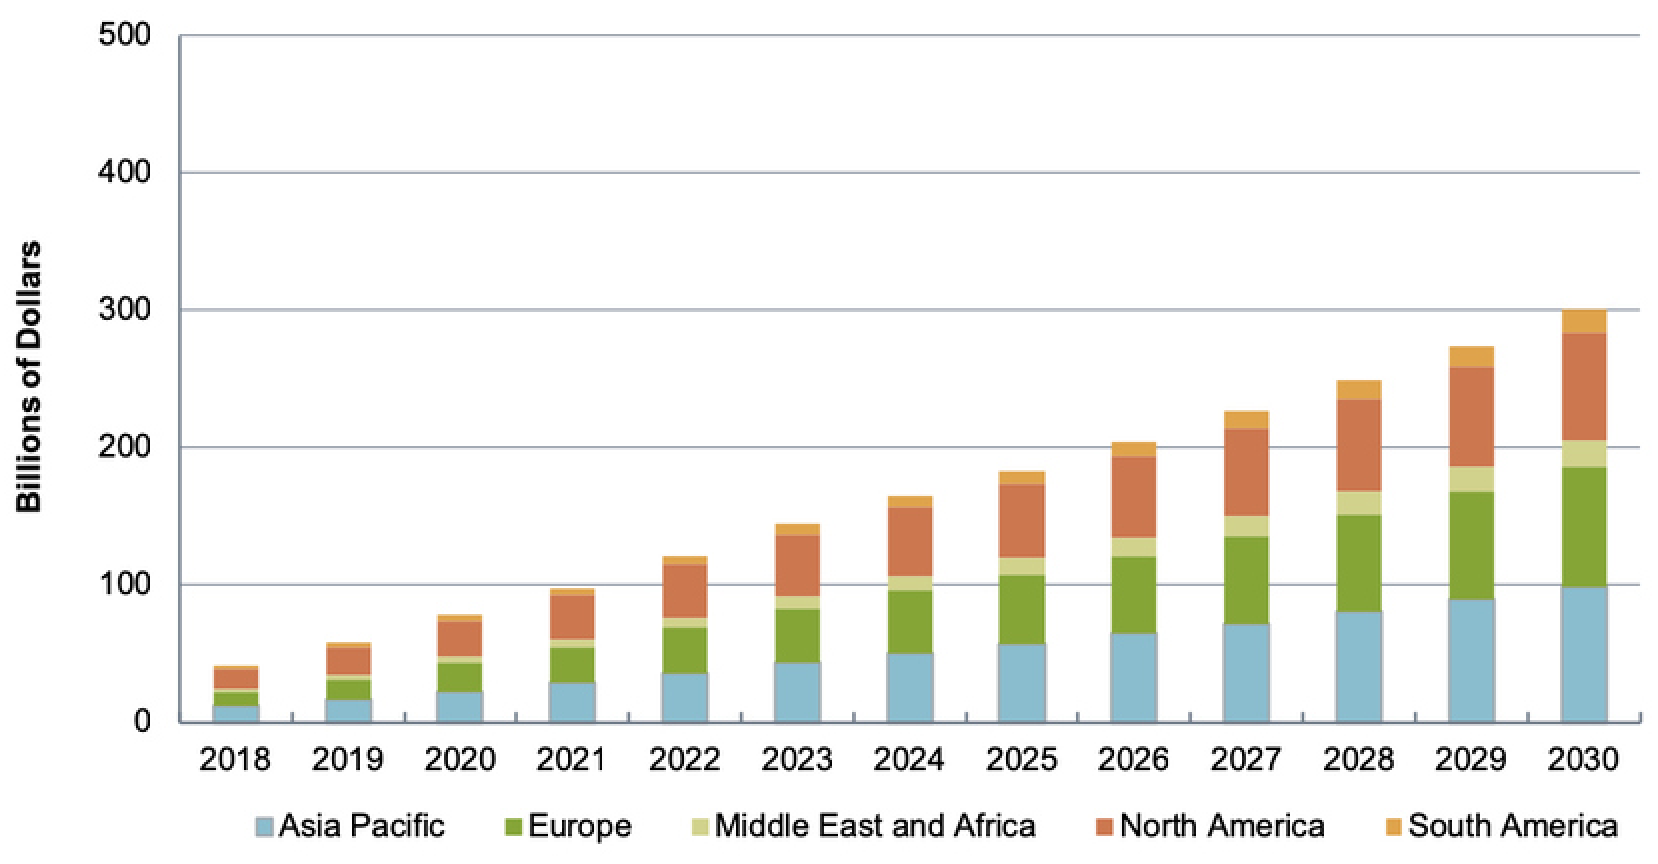
\includegraphics[width=0.8\textwidth,height=\textheight,keepaspectratio]{images/Banking_AI_Business_Value.png}
    \caption{The business value for the world market for AI in banking by region}
    \medskip
    \footnotesize\textit{Source:} "Artificial Intelligence in Banking Report", IHS Markit, 2019, p. 10.
\end{figure}

Even though, as previously mentioned, United States banks are leaders of Artificial Intelligence application, where companies earned additional \$14.7 billion in 2018 thanks to those technologies, experts expect that by 2024 the Asia-Pacific region will break out into the lead, as banks expect to earn and save, thanks to AI, around \$50.6 billion, while in 2018 those banks saved \$11.5 billion.
By 2030 it will raise up to \$98.6 billion due to demand in China (including Hong Kong), Japan, South Korea and Singapore.
\cite{ihs_markit}

According to forecasters, by 2030 banks in the whole world would be able to decrease costs by 22\% using Artificial Intelligence technologies. 
In numbers, this reduction can reach \$1 trillion.
\cite{trillion_opportunity}

According to Accenture, the amount of savings by 2035 will be nearly \$1.2 trillion.
\cite{accenture_ai_banking}

The most tangible changes will occur in units that have direct contact with customers.
By reducing amount of retail divisions, cashiers and security officers, banks cut costs by \$490 billion.
In departments responsible for data processing, analytics and reports, 
introduction of Artificial Intelligence will save up to \$350 billion in middle office and \$200 billion in back office.
In the US banking sector, more than 1.2 million of employees have already encountered AI, even thought they may not be aware of it.


Nevertheless, AI technologies should change structure of financial industry, making bank sector more humane and intelligent.


The profit for the bank is obvious, as it will result in significant cost reduce.
However, forecasts about employment in front banking are much less optimistic.
Recent study of Autonomous Research have shown, that AI can lead to 1.3 million employees losing their jobs in the United States and 500 thousand employees in Great Britain.

Former CEO of Citigroup, Vikram Pandit, who is considered as FinTech evangelist, assume that 30\% of bank employees can be replaced by Artificial Intelligence in near future. 
The threat of layoffs is real for existing bank employees.
Former CEO of Deutsche Bank told, that they intend to replace 98 thousand of workers with smart software solutions, while
Japanase Mizuho Financial Group will free 19 thousand of workplaces, third of entire stuff, by 2027. 
\cite{ai_reality_hype}


IHS Market assumes, that among bank employees, who can lose workplaces, the biggest risk is for B2C front-office workers, especially, cashiers, customer service, interviewers, clerks, financial managers, controllers and credit specialists.
\cite{ihs_markit}


Even though usage of Machine Learning for complex analysis is not an innovation, according to Vasant Dhar, Informatics Professor in New York University and founder of SCT Capital Management Hedge Fund, which has been applying AI for 20 years, foreign exchange markets are still a significant challenge for AI algorithms and modelling.
Complexity and variety of macroeconomic factors, which can have influence on inter-currency relations, crucially complicate analysis for foreign exchange markets, unlike regular stock markets that has been using AI and ML for a long time.

Main criticism of AI is based on lack of trust to results, as ML supposes Black Box analysis and finding interconnections in unpredictable ways. 
Therefore, most of the critics cannot accept prognostic findings to AI, as it processes data without building relationships
between cause and effect.

Despite rational enormous cost savings, a number of researchers are recommending to step off radicalism.
In their opinion, banks should be careful not to rely too much on new solutions.
Its effectiveness is extremely clear only in case of complementing human work, not replacing.
Therefore, introducing artificial intelligence, banks should be prepared at least to educate employees of robotized work process.
Large Dutch bank ING agrees with this position:
“We would like to use artificial intelligence in order to suggest more thoughtful decisions to our clients and to be more effective in decision-making, and not to replace workforce with AI”.
\cite{ai_reality_hype}


On this direction there is a temptation to improve the artificial intelligence, making its possibilities closer to human ones. 
Unfortunately, much still remains outside the perimeter of capabilities of modern technologies.
AI has a function of recognition, but not of cognition. 
It is wrong to assume that humans and machines can work on a same level.
It would be a long way, and it would require significant research until machines begin to at least approaching level of human performance.
Predictions regarding the timing of the creation of truly “smart” intellect are pretty vague.
\cite{ai_reality_hype}


Doubts arise not only in terms of timing.
Considerably more important are considerations of a generalized and even philosophical nature, for example, whether it is generally necessary to strive to model human thinking in its entirety.
The spheres of application of human and machine intelligence should coexist in complementarity, and not repression (or replacement)
In a number of situations, there are no simple tasks that can be solved purely algorithmically, but a human mind is needed to cope with them.
However, humanizing artificial intelligence deprives it of those strengths, for which, actually, human tries to create and swap himself with rational, algorithmic and objective source of actions and decisions.

Digital economics brings changes not only to operational bank activities, but also into relationships within community of financial institutions.

Research conducted by World Economic Forum together with Deloitte and Touché led to the conclusion that possibilities, which are being brought by Artificial Intelligence are an option only for the largest banks.
Since the main innovation concentrate on customer acquisition channels, then it is very likely to observe banking sector regroup — the dominance of large structures and the withdrawal from the market of small and medium structures.
\cite{ai_transform_disrupt}

However, researchers leave small companies a chance on survival.
Those assume that smaller companies have an option to specialize in certain directions, types of operations and specific clients.
Consequently, along with large banks, customer service in digital economics may be provided by small niche financial companies.
\cite{banking_ai_revolution}

The desire of benefit by expending of information base and Artificial Intelligence, which is the main data consumer, will lead to creation of monopolies — large alliances of financial groups.
The need of strengthening and enhancement of bank cooperation is required by increasing importance of analytical work, grow of risks of cyber-attacks and fraudulent schemes. 
The effectiveness of protection against criminals significantly increases in the conditions of sharing information about criminal patterns, sharing blacklists of companies and clients.

Nonetheless, transfer, control and usage of received data has to be settled down, including legal establishment.
Data owners, as well as clients, are interested in reliable control over data.
As a result, there is a need in obvious legal procedure of personal data transfer and its protection.
The transfer of activities to digital space creates entirely new risks and requires new methods of risk countering, which have not been worked out yet.

At the group level banks agree on a fact, that main route of development of banking is based on implementation of opportunities offered by digital economics.
Moreover, banks apply the latest achievements of computer technologies and software development, among them Artificial Intelligence, in individual areas of its work, replacing an employee with robot on routine repeating operations.
Nevertheless, banks are very careful about complete and deep technical restructuring, sending significant funds for studying the issue.
Regarding modern stage of Artificial Intelligence application and immediate prospects, I would like to cite The Financial Times:
8 years ago there was a talking robot in Santander Citi, but none of them is left in any of 13697 branches of the bank.
\cite{ai_reality_hype}

Even nowadays, banks are still focused on creating necessary conditions for AI transformations, including preparation of infrastructure, data, models and processes.
In addition to fields, that always have to be on the cutting edge, in order to gain advantage as a pioneer, 
changes are coming to more conservative spheres of financial services.
Despite the active usage of Artificial Intelligence, most banks have not had time to implement it globally yet.
According to experts, overwhelming majority of financial institutions noted usage of Machine Learning in one degree or another, but, as it had been noted by experts, only 20\% of respondents went beyond the basics of AI usage.
\cite{ai_reality_hype}

But structurally, banks were creating single open platforms, which provide general service for all domestic business customers.
Therefore, there is a need in relevant professionals, who would be able to handle and support platforms.

% !TeX root = ../../master_thesis.tex


\section{Artificial Intelligence in Operational bank activity}

Nowadays, banks are equipped with modern information and communication technologies.
At the same time mentioned technologies, including Fin-Tech software, have significant impact over existing financial institutions.
By surpassing operational limitations, those technologies become the main factor of transformation of both in a case of single bank, and in a case of entire banking sector. 
This results in a gradual increase of computerization of banking industry, leading to larger possibilities of application of artificial intelligence.

Significant volumes of information are being accumulated over financial markets resulting in data analysis being more and more relevant.
Some experts note, that markets are already emerging where data sharing is critical to competitive success and first movers are positioned to distinguish themselves by delivering better advice, constant presence, and curated ecosystems. 
Firms that lag behind are finding that their old strengths may not keep them as competitive as they once were.
\cite{ai_transform_disrupt}


\subsection{Artificial Intelligence in Investment Banking}

The pioneers of application of modern Artificial Intelligence and related technologies are, obviously, investment banking companies, which had to apply modern solutions in day trading algorithms. 
Those companies target Machine Learning and Natural Language Processing in order to use it for data, news and content analysis.
For them the most popular source of alternative data are news aggregators, expert networks and search query indexers.

Most of the asset managers and hedge funds specialists suppose that according to existing competitive dynamics, the trend of research disaggregation will continue even in regions not covered by MiFID II, legislative framework instituted by the European Union to regulate financial markets.

There is a popular opinion, that during researches investors would rely less on investment analysts. 
Some expect major changes in investment research market, as investors would need more data for support of AI and Machine Learning technologies.
On conducting researches, portfolio managers would rely less on investment analysts and more on internal solutions, data suppliers and solutions suppliers.
\cite{future_of_trading_technology_2024}


\subsection{Artificial Intelligence in Commercial Banking}

As for commercial banking, the status of AI integration highly depends on bank size.
All over the globe major financial players have been developing solutions based on Artificial Intelligence for the last 60 years with the various levels of success.
The situation has been especially progressive for the last 10 years.
In general, over 70\% of large global banks studied and have implemented AI for front-office or back-office functions.
\cite{deloitte_thriving_in_ai_era}

However, as for middle-size financial institutions, situation seems pessimistic.
While largest banks have been developing AI strategies, creating teams and projects in place by investing billions of dollars, for midsize banks AI was not even on the radar.

In comparison, while large banks have been investing majorly since 2016, in 2020 less than 20\% of midsize, or less, financial institutions invested in, implemented, or at least planned to apply AI.
What is even worse, only 2\% of those have deployed chat-bots, Machine Learning or other Artificial Intelligence technologies.
\cite{ai_transform_disrupt}

The main reason is in AI capital limitations.
Even though, those technologies can be independent of existing business structure, the last are highly dependent of capital investments.
Therefore, large financial institutions Banks that act now can capitalize on the power of automation and intelligence to truly transform their organizations.


Midsize and smaller banks and financial institutions have to compete with mega-sized counterparts without R\&D budgets.
What is even worse, the gap between large and non-large institutions only increase, because of how AI works.
The longer AI operates, the smarter and more useful it becomes.
As a result, the longer financial institutions wait, the harder it becomes to catch up. 
Financial institutions that start early gain a head start of months—even years—to gather data and “train” their self-learning, intelligent applications. 


Consequently, currently Artificial Technologies are available mostly to big players.

However, for midsize and smaller institutions not everything is lost, as there is a third-party option.
Machine Learning and Artificial Intelligence is highly used in start-ups, and application of solutions of those may save capital for research and development, and would allow applying tested solutions.
Secondly, most AI start-ups are small. 
Pilot programs and third-party innovation labs give banks and credit unions a chance to test, learn and refine your AI initiatives for a relatively small cost, before seeking funding for full-scale roll-outs.


However, one of the most important question of this analysis is what should banking acknowledge as Artificial Intelligence, what are its forms and possible use-cases in practice.

Currently, there is an extremely wide range of opinions.
Due to lack of unified theoretical platform of banking services, forecasts of development of banking institutions based on AI differ drastically and are based on business strategies of every single bank.
Nevertheless, there are 2 main routes of development.
First route is about focusing on cost reduction by workforce replacement and automatization of repeating routine operations without significant reformations of existing organizational structure.

On the other hand, there is a perspective in new digital technologies, which may allow inventing and introduce qualitatively different business models based on new market challenges, and, as a result, developing brand-new sources of income.
\cite{ai_reality_hype}

Nevertheless, in general, Artificial Intelligence in banks can be used in lots of areas.
From bank's perspective AI is needed from its ability to harness bank data in three key ways: to analyze, to act, and to improve by self-learning.

Systems of Artificial Intelligence were developed for automation of clerical workload, other routine paperwork, processing of various data sets.
In the digital age, banking transaction operations are just a form of abstraction over data transfer and storage.
Even though largest banks prefer to save more traditional organizational structure, they actively embed digital technologies in everyday practice.
Even though, banks prefer a less risky way, Artificial Intelligence application is applied in all bank fields, on all office levels and has to be precisely analyzed on each of those levels.



\subsection{AI in Back office}

Both Artificial Intelligence and Machine Learning may have significant influence on entire Back Office of Commercial banking.
Back office is known for enormous amount of repeating actions due to Execution, Clearing and Settlement process.
Therefore, the primary appliance of AI is in automatization of repeating routine operations.
Automated solutions, that automatically builds behavior patterns is ideal of Back Office, as it initiates high back-office efficiency via automation.

Ironically, this case is the case, when human intervention can impact more negatively, than positively.
For repeating actions, for example, calculations, in which there is no responsible decision-making, artificial intelligence suits the most.
“For repetitive tasks without variability (in middle office, in back end) for clearing/settlement/operational processes that are not particularly in need of smarts, 
then AI approaches are great,” says Pascal Bouvier, a venture partner at Santander InnoVentures, a fintech venture capital fund of the Spanish bank that invests in early stage Fin-Techs including those focused on AI.
\cite{ai_reality_hype}


Special attention of applied automatization is directed into processes, that require large amount of work, but offer low profitability.
McKinsey shows as an example of JP Morgan, which had started using chat-bots for IT service request automatization.
In 2017 1.7 million of requests where processed this way, which is equal to yearly full-time workforce of 40 employees.
\cite{ways_ai_transforming_bi}


In fact, it is possible for bank to transfer to robotic solutions such operations as:
\begin{itemize}[noitemsep]
    \item Payments processing of legal entities and individuals
    \item Processing of unidentified payments
    \item Customer data change based on statement
    \item Editing credit agreements based on individual statements
    \item Document processing
    \item Credit underwriting
\end{itemize}

Another popular application is processing of incoming documents.
Modern scanning programs can recognize standard documents and transfer them to performers.
Naturally, this kind of programs contain special filters, which direct documents, that do not fit into specific characteristics, for expert review.
Moreover, modern systems allow recognizing most typical types of documents and fill it using typical forms.
This allows a practical usage of these tools for legal office and even compliance control divisions.
As a result, activity of institutions become aligned to established regulations.
However, undeniable benefits of automatization based on artificial intelligence can be fully achieved and felt only in case of continuous update and upgrade of technological base.
\cite{banking_ai_revolution}

As an example of direct application, it is possible to refer to remittance matching solutions, that improve straight-through processing.
As an example, Deluxe offers AI based payment to remittance matching, which should shorten Days Sales Outstanding resulting in a same-day posting
\cite{deluxe_ai_remittance}

% if more needed: https://internationalbanker.com/finance/artificial-intelligence-storms-back-office/


\subsection{AI in Middle office}

In comparison to Back Office, where AI may be used primarly for infrastuctural changes and evolution, Middle office is open for the biggest cost cuts and optimizations.
According to researches, Middle Office alone can save \$217 billion, around 50\% of all cost savings available by AI for banks by 2023.
\cite{trillion_opportunity}

The reason for this is hidden in a definition of Middle office by itself.
Middle office is comparably new division of a commercial bank, and usually forms a bridge between customer flexible Front and strict and executive Back office.
Hence, Middle office operations by its nature are structured and documented, but have a certain level of statistical disturbance.
Thus, it makes Middle-office the most interesting and sensible target for AI development for commercial banking.

Importance is based on a combination of possible backfire of operation logic and unpredicatable patterns, that can form in everyday work.
This leads to, probably, the most obvious area for AI in Middle office — Credit Scoring.
AI in this case allows calculating credit scores not only based on known mathematical models, but to find out new, previously unknown patterns.
As an example, credit risks for private clients can be analyzed based on user's digital footprint, that can reach enormous amount of data.
Moreover, this may be true for clients, who have no credit history, or very old credit history, as it would allow to set a credit score based on a data of other clients.

Secondly, AI has a major usage in Anti-fraud.
Practically, it has the same reason to use as for Credit Scoring — it is possible to unite existing models with unpredictable patterns.
In this case model can analyze not just payment data, transaction history, transaction time and location, but in a various combinations based on possible patterns of transactions of other users.
Additionally, AI supports and provides face recognition systems.
As for ATMs, all actions can be guaranteed by face recognition.
It is true for Internet Banking for customers and CRM for bank employees as well.

Furthermore, the same reasoning is true for both KYC and AML compliance.
In general, Artificial Intellegence brings multiple possibilities for KYC and AML, such as unified pool of data, probabilistic matching, progressive evolution, self-training and pattern-based analytics in conjunction with rule-based.
Moreover, these features allow using AI in Risk Management, for credit and risk underwriting.

% proof: https://www.h2o.ai/resources/solution-brief/know-your-customer/

Based on existing estimations, around 20\% of digitalization projects are targeting cost reduction or productivity increase.
Most of those are targeting on potential risks recognition and minimization of risk consequences.
\cite{ai_reality_hype}

Artificial intelligence may frame out unlawful behavior, including non-stereotypical one.
By processing big data artificial intelligence may find out an evidence of fraud or illegally money laundering attempt.
The most simple way, but still significant, criminal pattern identification and revealing unlawful activity.
 
Artificial Intelligence can cover large databases and catch patterns, which hide from human attention.
Even more complicated approach of AI usage is educating to identifying market noises.
As a result, more advanced technologies allow discovering and determine people and companies with elevated risk for banks, allowing to build safer relationships with them in future.

Crimes in virtual banking are evaluated in \$600 billions yearly.
Artificial Intelligence and Machine Learning as main instruments for risk management in banking practice are mainly oriented on financial crime prevention.
This is much more efficient, comparing to complicated processes of damage compensation and financial crime evidence confirmation search.
Mastercard, for example, was able to reduce attacks on customer accounts by 80\%.
\cite{ways_ai_transforming_bi}
 


\subsection{AI in Front office}
\label{subsec:ai_front_office}

Numerous Financial Instituations are leveraging AI-driven chatbots and algorithms to support existing customer service channels with faster, more consistent intelligence.
One of the common thoughts on AI application in Front office are Biometrics.
Biometrics are widely represented by various recognition systems for much safer authentication.
Voice recognition is used to determine client by voice, facial recognition technologies, which are based on ML and AI, help to determine a client or to check correctness of client's photo data.
Similarly, Computer Vision technologies allows to determine the authenticity of physical signature.
However, it is more correct to consider biometrics as an input for Anti-fraud systems. 

As a minor use case, Front Office is interested in offering Personalized financial products, but this solution can be interesting for financial aggregators and Banks-as-a-Platform, but both those forms of financial institutions are comparably immature.

Even more rare is an application of AI in case of Robotic Advisors and Algorithmic trading on a consumer level.
However, it became more active since last year.

This is an alternative to communication with financial consultants in order to create and manage investment portfolios
with stocks, bonds and other assets.

In just a few minutes, according to the set parameters, the robot advisor can assemble a balanced, by industry and company, investment portfolio, taking into account the available investment amounts, with the optimal ratio of risk and profitability.

It is believed, that those systems can create accurate forecasts for stock market environment, due to possibilities of
automatic collection and analysis of the state of foreign exchange markets and latest economic news.
This allows client to invest into tools with the lowest risk.

Robo-advising became a powerful alternative to financial consultants in basic questions, related to banking, financial management and cash transactions.
The portfolio in the US financial markets, which is now being managed by robots, have already reached \$1 trillion in 2020
and rapidly increases, expecting to make up its volume up to \$2.85 trillion in 2025.
\cite{europarl_roboadvisors}

Going further, AI can be widely used not only for helping clients with investments, but in entire Individual Banking.
Standardized financial products and services for wide range of consumers cannot satisfy needs of modern client.
Modern clients require personified conditions for accounts, loans and other services. 
Without individual approach it is impossible to implement, therefore, one would need Artificial Intelligence as well.
Nowadays, every financial entity develops and offers between 10 and 20 financial products.
For developing such products banks need a team of professionals.
Developing hundreds of thousands of personified offers for every bank client is, by fact, impossible without help of Artificial Intelligence.
According to statistics, nearly every person has between 2 and 5 electronic devices, which can connect to internet, use various messengers or social networks.

Naturally, every internet user leaves enormous volume of data after himself.
Analyzing that personified data effectively allows creating various unique personified advices and offers.
Algorithms of Artificial Intelligence, theoretically, can collect client information, analyze and generate individual personified offer.

As a result, whole service industry becomes more and more personal.
Screening social networks profiles, collecting GPS or any other position data allows classifying client and to create his social portrait.
Obviously, from bank's side, it allows to effectively determine credit rating for every client.
At the same time, as an example, if one works in an agricultural field, bank can suggest and recommend various products connected with harvest insurance.
As for small business, analyzing supply chain and contragents of that business, bank can at the same time analyze seasonality of payments and more accurately predict time ranges, during which client liquidity can drastically decrease, or possible cash gaps.
This knowledge allows bank to operate more effectively and saves business from a useless hassle.

At the same time, case of Conversation Banking is extensively developing and has to be precisely analyzed.
Conversation Banking for the last 3 years became extremely popular.
Among the largest U.S. and international banks, the greatest focus today is on conversational interfaces, such as chatbots and virtual assistants.
\cite{deloitte_thriving_in_ai_era}

The main purpose of Conversation Banking is a client communication.
Nowadays, there are general purpose AI programs, that are able to speak to people.
Having a chat-bot call assistant for common problems allows bank to extend it into artificial personal assistant, including financial one, that can help a bank client using his and only his data.

Chatbots are one of the most effective ways to answer questions from employees and customers.
Client can call to a bank and talk about his problem, but due to the fact, that this problem can be categorized, a client can talk to bot, that can help client to solve his problem and tell about some problem related services.
Moreover, it can analyze client needs and immediately provide various financial recommendations.
Of course, that can be presented with any form of communication, both with SMS, internet messages or voice messages and calls.

But there is even more interesting point of view.
Based on the various researches, banks that are targeting teens and younger adults has to take to its concern, that younger people are not used to talk over phone, but to contact via messengers. 
Therefore, banks have to develop text chat-bots, and on various platforms, including bank's website, bank's mobile application, and chat-bots for application, where those people prefer to use, like Facebook.

In addition to chat-bots, banks can use voice assistants.
According to him, the assistant will help users in solving financial and everyday tasks — money transfer or reserving a table in a restaurant.

For example, Apple Siri, Amazon Alexa and Google Assistant are tightly coupled into everyday life of modern people and access to such fields of can result in an extremely high level of interaction between bank and client, and, therefore, increases client's loyalty. 

Bank's client can ask in this case various general questions and receive answers immediately.
For example, client can ask what payments were done with debit card last week, 
level of debt of a credit card and when fixed-term deposit ends.
As a result, client doesn't spend time looking for information on bank's webpage, sorting history in mobile or web app.
The assistant has another area of usage as well. 
For example, using an installed app, that is able to recognize products on store shelves, assistant can display cashback amount, which would be returned to the client after paying by credit card.

As a result, client communication is expected to outlive vitaly crucial challenges. 
Firstly, there is a growing competition over clients, both in attraction of new and in retention of old ones.
Secondly, ready-made technologies may allow to execute this much more effectively and with lower costs, then an operator.
Basically, almost all banks replace communication employees with a program — the chat-bot.
Usually this transformation is being done painlessly for a bank, as in most cases a foundation already exists.
In recent years operators were building client communication based on a script, scenario of a dialog.
In case of more complicated talk, operator have to transfer a talk to a manager with more responsibilities.
Based on research, modern chatting solutions can not be distinguished from an alive person by 60\% clients.
Chat-bots are attractive for business by providing consistent access to bank information with an immediate feedback, which is extremely important for the client.

Response delayed by 5 minutes decreases chances to create long-term bonds with a client by 10 times, resulting in building bonds with a bank, that answered the call, as in this case client feel himself important. 
Nevertheless, it is still important to leave a possibility to contact an alive employee, as 79\% of respondents would positively react on a conversation with a human,
while 74\% negatively react, if they would have a conversation with a machine, without a possibility to have a contact with a human.
However, modern programs may transfer communication to an employee, who has much more possibilities to handle a non-typical talk.
Client is important for a bank in case if he is using bank services on a regular basis, and constant contact is a reason of 70\% of purchases of banking services.
Chatbot, as a universal worker without breaks and competitors, especially for big banks with large client base, which bank has to be in a constant contact with.
Nowadays, such robots to a large extent are replacing call centers, mailing centers and in certain cases marketing divisions.

Swiss bank UBS, which is in Top 50 by assets, developed service Ask UBS to serve companies which specialize over managing client finance.
Offered service allows receiving advices in wide range of questions and financial markets analysis.
Moreover, it works as an educational service, clarifying definitions, giving definitions to acronyms and translating professional slang of the financial market.
According to UBS representative, bank intends to turn Ask UBS into a common instrument, which could be “secure, compliant, and trustable for clients.
\cite{ways_ai_transforming_bi}

Correctly developed program may not just execute multiple routine functions, but have an ability for self-education and self-correction.
Some specialists assume this would not be any burdensome development, if software developers didn't receive overcomplicated requirements.
However, extremely complicated solutions supporting multiple platforms and self-learning may be pretty expensive.
Therefore, most banks start exploring the digital world of chat solutions with simple virtual agents, which is mostly based on scripting and scenarios.

Another important direction of client communication improvement is the personalization of products and services.
Personalization is one of the main, if not the main, instruments for competition in banking sector.
Previous criteria of competitiveness, as price of banking products,  service delivery rate and accessibility, are fading out in significant extent, especially due to the fact of equalizing of competitors due to equivalent access to modern technologies, leaving no place for tangible superiority.

Competition over bank client moves towards digital solutions with the priority to develop client adapted, demand-based product, to form convincing recommendations, up to ready-made solutions, based on client needs, thoughts and expectations.
Banks obtain possibility to influence actively on client behavior by using large amounts of data.
By processing that data, artificial intelligence receive an option to offer client personified product on best suitable user conditions, as it, obviously, considers client's targets and financial possibilities.
It is common for such products to get ahead of client wishes, resulting in forming request by consulting and clarification.
\cite{ai_transform_disrupt}

Santander bank even instituted an award for developing a program, which would allow joining banking products with client needs.
\cite{ways_ai_transforming_bi}
In this part of banking the importance of consultants and intermediaries in relationships between banks and clients is increasing.

Naturally, conditions of digital economics allow for a robot to be the consultant, which would make recommendations about better products, institutions and services oriented on specific client.
This results in a trend of separating it into independent activities without binding to a single financial company.

Possible options of activity for general purpose solutions are much wider, as such solutions are not only based on bank products and services, but those can offer interaction with companies with more favorable conditions.
High level of personification of service and demand for intermediate service providers may even lead to the extintion of traditional forms of product offering, which is currently based on each product separately, for example, debit cards, payment systems, loans and saving accounts.
Instead of traditional offering, digitalization allows for development of universal financial service, which would implement all financial client requirements in a single integrated service, and what is more important, in way which would fit client needs the most.
One more step towards banking automatization is remote customer service for a certain range of operations.
Such possibility can be offered by a solution, identifying client by specific features — facial features, voice features or finger capillary network.

There are even more exotic options. 
For example, one Japanese researcher suggest using individual person's blinking behavior.
British bank Halifax conducts test of a special bracelet, which would register individual heartbeat features.
\cite{ways_ai_transforming_bi}

Some of those technologies have already been tested in production for financial operation. Most known example is the Apple Pay on iPhones, which uses facial recognition not only for phone unlocking, but also for executing operations via Apple Pay and other digital wallets.
Specialists claim that ways of person identification are becoming more complicated. 
On the other hand, those technologies at the same time become much more reliable and stop being exotic.

Google Intelligence predicts that by 2021 1.9 billion of bank clients would use biometric data for remote services.
However, there is still no large demand by banks for such remote forms of service, even though those technologies of identification have been developed long time ago and even tested by bank security services.
This is mainly due to lack of guarantee for operation to be voluntary, without any unlawful influence and there is no satisfying solution for such problem yet.



%\section*{Conclusions}
Artificial Intelligence has already become a leading driver for technology innovations in banking sector.
It has already been developed enough and definitely reliable in everything regarding risks, confidentiality, human factor and marketing strategies.

Nevertheless, AI has already changed financial business and will change it even more in near future.
The vast majority of actions, that are being done both in back-office, middle-office and front-office by employees can be automized and algorithmized.

\begin{table}
    \centering
    \caption{Fintech AI Use-cases}
    \begin{tabular}{| c | c | c | c |}
        \hline 
        \textbf{Divisions} &
            Front office & 
            Middle office & 
            Back office \\ \hline 
       
        \textbf{More mature} & 
            Conversational banking & 
            Anti-fraud, KYC, AML & 
            Credit underwriting \\ \hline 
       
        \textbf{Less mature} & 
            Biometrics & 
            Legal and Compliance &
            Smart contracts \\ \hline 
        \textbf{Savings} &
            \$199 billion &
            \$217 billion &
            \$32 billion \\
        \hline 
    \end{tabular}
    \medskip
    \source{Own study, based on: Lex Sokolin, Matt Low, "\#Machine Intelligence \& Augmented Finance", Autonomous Research, p. 29.}
\end{table}

The main interest for banks is in application of AI in front-office and middle-office, as it will lead to significant cost reduction, up to \$400 billion in 2025.
Banks use AI in front-office for identification and authentication of clients, in order to imitiate alive workers with chat-bots and voice assistants, to deepen relationships with customer, increase engagement, and to offer personalized ideas and recommendations.
Additionally, AI is being used in middle-office.
It allows detecting and preventing frauds with payments, upgrading processes connected to anti-money laundering processes and detection for know your customer control systems.
Those sources of income, which have already been transformed by AI, show the valid way to use this possibility.
Nevertheless, those strategies show that banks have to create holistic strategy, which would connect and cover multiple scopes of banking, sources of useful data, third-parties and employees.
\cite{autonomous_next}

However, with all the advantages of modern software, forecasts of full robotization probably won't be realized, as in near future it is unlikely for a program to replace a person.
\cite{deluxe_mid_size_banks_risk}

In order to integrate the foregoing into existing banking service it is necessary for banking platform to support it.
Obviously, those platforms, which current banking stands on were developed around 15-30 years ago, or even more, and this makes integration of modern algorithms almost impossible. 
This is why modern banks are now puzzled if it is possible to reengineer their software in order to have an effective possibility to embed Artificial Intelligence and Machine Learning in its banking platform.

Nevertheless, it is extremely important to remember, that automating workplaces doesn't always lead to dismissal of workers.
It is important to create retraining programs, that would allow existing employees to obtain new skills in fields,
that are out of risk of automation, in order to decrease automation's influence on labour market.

Increasing number of internet users, availability of smartphones and other handheld devices, and rapid development of mobile internet forms new users' habits and behaviors.
Social network users and mobile app users are more and more focused on getting instant results and target specific actions with the lowest amount of clicks possible.

However, the need of receiving high-quality financial services and personal consultations hasn't disappeared: people are still calling to call-centers.
Even though remote banking service systems are rapidly developing, number of phone calls recently significantly increased. 

Nevertheless, there are good news for banks that have yet to embark on their AI journey. 
Making progress in AI does not require an unbearable effort.
It typically begins with identifying your organizational goals, readying your data and finding the right partners.
Nonetheless, even medium-sized and small banks have to investigate this topic by now, as in future, gap between AI users and nonuser will only widen.







% Chapter 3
% !TeX root = ../../master_thesis.tex

% Chapter 3
\chapter{Chat-bots as a new approach} \label{chat_bots}

% !TeX root = ../../master_thesis.tex

\section{Chat-bots. Overview and theoretical aspect}

Chatbot — is a complex multivariate algorithm, which is able to perceive information in the simplest and most understandable for the people form — dialogue.
In the process of communication with a person, chatbot analyzes lexical data and forms logically correct answers.
As a most common example, with the help of chatbot, now it is possible to order pizza, find suitable flight and hotel, set necessary system parameters, set an alarm clock or find up-to-date weather or sport information.

Chatbots from a highly specialized, most often non-profit, entertainment turn into a tool.
Previously, chatbots were considered as a highly specialized solution, as an entertainment and as a proof-of-concept.
Nowadays, it is being understanded as a necessary tool for all kinds of messengers, social networks and applications.

Chatbots are recreating whole IT ecosystem landscape.
Even though for the user it is just a companion program that is designed to help, on the other side there is always a complex system, based on a couple of AI technologies.
Obviously, it is entirely new industry of service and assisting.

Generally, chatbots perform three main groups of tasks:
\begin{enumerate}
    \item Executing routine common operations, that could be translated to a specific algorithm
    \item Search and data aggregation — chatbots are able to collect material on a given topic and form it in a certain way
    \item First line of customer service — in addition to providing advices on goods and services, chatbots can focus user attention or entertain him, although most of the chatbots can only answer to basic questions.
\end{enumerate}

Rule-based chat-bots with pregenerated and specified workflow exist from the very beginning of IT.
However, AI-powered solutions are comparingly new.
The biggest impact in the last decade was done by Apple and its voice assistant Siri in 2010.
It would be impossible to create such solution without Natural Language Processing and Machine Learning technologies.
However, the main reason was due to full control of operational system they were able to build a market.

The second wave of AI popularity was due in 2016, when Facebook made a bot platform, which allowed to create AI-powered bots inside social network.
This showed practical importance of such technologies and was a main driving force of further practical applicaton on AI in front-offices in various industries.
As a result, apart from being the biggest social network, with 3 billion monthly active users \cite{facebook_statistic}, and an important channel of customer communication, Facebook obtained a massive influence on chatbot market and is one of the main catalyst of growth of this market.
Moreover, Facebook invested significant funds into development of speech technologies, creating both toolkits for developers and developing and new sells channels, which made AI chatbots with NLP even more accessible.

Starting from 2017 banks, various financial and insurance companies started showing interest toward chatbots with AI.
Moreover, same year some of them developed and integrated automatic communication technologies in client communications.
The first global banking chat-bot hit was Bank of America's Erica in 2016, an AI-powered financial assistant embedded in its mobile banking app, recently passed 20 million users with more than 105 million interactions.
As another proper example is a Citi Bot by Citibank, which was developed in 2018, received a hude success among Facebook users.

In 2018 volume of the global chatbot market reached \$1.27 billion.
Moreover, experts expect that starting in 2024 global spending on dialog services with Artificial Intelligence will be increasing by 34.75\% and will achieve \$7.59 billion until the end of 2024.
\cite{gartner_chat_bots}

Even though by the end of 2021 the quality of chatbot implementations was on a pretty low level, its popularity is growing rapidly.
On the other hand, the positive effect will be brought by massive consumption of services of devices with NLU support, for example, smart speakers, or voice interfaces for mobile applications.
This leads to popularization of voice control, due to its expluatation convenience and possible automation of routine processes, as those speakers usually can work as a voice controlled assistant.
Henceforth, by 2025 existence of talking chat-bots, de-facto, will become the norm for most of the internet services.
\cite{accenture_chatbots}

Chatbot technology is quite in demand by marketing departments of various companies for quick contact with potential customers, as well as online customer support organizations.
Chatbots act as a customer manager services or as a support specialist.
Company, which uses this technology, can obtain both an advantage, for example, reduced staff costs, and a disadvantage — outflow of clients who do not want to conduct a dialogue with the "computer". 
Consequently, chat-bot technology allows optimizing business-processes and find out reasonable compromise in simplifying client interaction with bankers with simultaneous increase of level of service and cost reducement on call-centers and SMS notification services.
Dialog imitation should occur in a familiar and comfortable for client environment, and at the same time client should receive choice of services which previously wasn't available via website or remote business service systems, so it could store and raise client loyalty.

Unfortunately, text recognition and natural language processing are an avant-garde frontier of Artificial Intelligence, and it still has to be brought up to an acceptable level.
Popularity of promising, according to multiple companies, of so-called interface bots, that are based on Social Network platforms, for example, Facebook, do not provide high-quality imitation of live conversation and do not maintain customer loyalty.
Those conversational bots are usually being criticized, especially its more primitive analogues,  as they still have limitations to have a mindful dialog.
Discussing issues clients are still in need of sense of live content and due to this the most promising direction is the development of conversational chat-bots, but only given that there are wide possibilities of language processing and analysis.
It would be extremely hard, but still possible to create a true chat-bot, that would be able to imitate human speech with high quality.

This solution will significantly decrease load on a call-center and keep the possibility of live dialogue in specific corner cases.
Additionally, this technology allows to create a specific subtype of chatbots, although it is more common, as it is being developed and supported by major companies of IT market — personal assistants.
Hundreds millions of people are interacting with personal digital assistants on such platforms as Google, Apple, Amazon, Facebook and others.
Digital Assistants are a specific subtype of chatbots, although it is more common, as it is being developed and supported by major companies of IT market.
Hundreds millions of people are interacting with personal digital assistants on such platforms as Google, Apple, Amazon, Facebook and others.
Textual and voice communication with user makes the transition from Graphical User Interface towards Conversational User Interface, which can be the key trend for the coming years.

Textual and voice communication with user makes the transition from Graphical User Interface towards Conversational User Interface, which can be the key trend for the coming years.
Many messenger apps, for example, Facebook Messenger, have public APIs — programming interface, which allows creating chatbots.
Companies can use those apps as intermediaries in order to increase performance of its employees.

Additionally, those can be a new channel for client service, either via corporate website, or by some new service channel.
Uber allows to order a car via Facebook Messenger.
But extremelly important is the launch of Amazon Alexa, that can be used by third-party companies for customer communication, as well as integrated into different user devices, like smartphones, smart speakers and any other devices with sound input, sound output and internet connection.

Nevertheless, chatbots are not just a simple frontend.
Firstly, banks can use same chatbot communication channel for notifications to increase level of client engagement.
In general, live chat can be used as a direct client communication channel with clients.
Information on product specs and services, contact info, payments proceeding, financial recommendations.
Secondly, large amount of client data allows making targetized, individual decisions and solutions.
This is a strong strategical advantage, as correct account information would allow more precisely offer personal recommendations.
Moreover, large amount of client data allows making more targeted decisions without using exclusively strategic approach. 
Account information and its nature allows more correctly approach personal offers.

Chat-bot is not an end in itself, but an instrument for checking and testing.
The only practical sense in chatbots are in costs reduction, not in profit generation.
On the other hand, high growth rates of chatbot market with NLP technologies is due to early stage of its formation.

Among the main problems, hindering the use of this technology, the main problem is poor user awareness of functionality, quality and convenience of services.
However, developers are trying to eliminate those disadvantages by launching various interactive features.
Despite having the greatest prospects in reducing costs for call centers and other support services, this technology has a great advantage in direct customer services.
Digital assistants would be able to make catalog navigation easier catalogs and offer users desired products.
Since local business is aggressively integrating Artificial Intelligence, future increasing costs of development of chatbots is just a matter of time,
as it would significantly decrease costs on customer service services.

Significant change is expected in Asia-Pacific region due to large amount of people and historically smartphone-oriented digital market.
Scientists of Temple University and Fudan University conducted a study among 6000 clients of financial service company.
All clients were talking either to chatbots or real people without expirience in sales.
Disclosure of the “identity” of the interlocutor was carried out at the beginning of the conversation or at the end, 
after the purchase.
Moreover, in several groups the “identity” was not disclosed.
AI turned out to be 4 times more effective than an ordinary unexperienced employee. 
However, if client founds out the company uses a chatbot before buying, the sale chance drop by more than 79.7\%. 
According to researchers, these results shouldn't restrain usage of chatbots.
AI has undeniable technological advantages, which allow reducing prices by reducing the cost of manual labor.
In addition, marketers would have to take this research into account and increase customer confidence in chat robots. 

The main feature is that chat-bots require same decision-making system as any other frontend, and is dependent of every single client.
This, in its turn, receives the biggest profit from PSD2 and Open Banking Initiative.

In order to implement such an automated conversational solution banks can either develop their own solutions from the very roots, use existing available instruments for individual custom solutions, or to apply available third-party options offered by specialized companies.
Current stage of ML technologies allows for companies to access NLP with considerably low costs for own implementation.
Modern programming technologies have various technologies and programming libraries for creation of NLP systems and many companies for advanced support.
Among most promising open-source solutions are DeepPavlov.ai and Rasa.
Those allow creation of own Natural Language Processing systems based on community support.

On the other hand, there are a lot of NLP start-ups, that focus on AI chatbots of various complexity.
Among those are LiveChat, Kore.ai with BankAssist, Kasisto, Morph.ai, Imperson.ai, Streebo, Creative Virtual and Artificial Solutions.

What is even more important, large IT corporations have their own solutions, resulting in easier form of integration with existing infrastructure.
Among those are IBM Watson, Google Dialogflow, Amazon Lex, SAP Recast.ai, Baidu KITT.ai, Facebook Messenger Platform.
The leader of those is currently Microsoft, which has Azure Bot Service, Semantic Machines and LUIS, Microsoft Language Understanding Intelligent Service.
Proper analyzes of possibilities require proper classification of chatbots by features.

\begin{table}
    \centering
    \caption{Chat-bot solutions with NLP AI}
    \begin{tabular}{|c|p{10cm}|}
        \hline
        \textbf{Open-source} & Rasa, DeepPavlov.ai \\
        \hline
        \textbf{ML\&AI solutions} & LiveChat, Kore.ai with BankAssist, Kasisto, \newline Morph.ai, Imperson.ai, Streebo, \newline Creative Virtual, Artificial Solutions \\
        \hline
        \textbf{IT Corporations} & IBM Watson, Google Dialogflow, Amazon Lex, \newline SAP Recast.ai, Baidu KITT.ai, \newline Facebook Messenger Platform, \newline Microsoft LUIS, Microsoft Azure Bot \\
        \hline
    \end{tabular}
    \medskip
    \source{Own study}
\end{table}


Firstly, by types of interaction.
User can interact with chatbot either by voice, or by text.
The same is true for chatbot, as it can answer either by generated speech or generated text.
\begin{itemize}
    \item Text
    \item Voice 
\end{itemize}

Secondly, by front platform, by form of user interaction:
\begin{itemize}
    \item Application 
    \item Third-party messenger
    \item Operating system
\end{itemize}

The reasoning behind this is in a possible platform of interaction with user.
Chatbot can be in a form of either part of mobile or desktop application, or as a part of web application.
Obviously, in this case user has to know and have access to website or mobile application for proper interaction.
Secondly, chatbot can be based on a third-party messenger, such as Facebook Messenger.
Thirdly, chatbot can be integrated with an operating system assistant.
For example, with Apple Siri on iOS and macOS devices, Cortana on Windows devices or Google Assistant on Android devices.

Additionally, we cannot ignore different forms of ownership.
\begin{itemize}
    \item Software-as-a-Service
    \item Internal development
\end{itemize}
Banks can use chatbots both using third-party tools, where chatbot ownership is on a side of third-party service, or as an internal tool with internal development. 

It should not be ignored, that chatbots can be used and developed differently for different end users.
By end user those can be divided to:
\begin{itemize}
    \item Customer-oriented
    \item Employee-oriented
\end{itemize}

The last and, probably, the most important internal classification is by decision-making process:
\begin{itemize}
    \item Rule-Based
    \item Machine learning
\end{itemize}

Rule-based chatbots are comparingly simple, as those are being built by a set of branch algorithms with limited number of options.
Machine Learning based chatbots, in its turn, can adapt to everchanging environment and create new answers, notifications and other forms of interaction based on a single client or a group of clients.


\subsection{Structure}

Structurully, chatbot can be divided into 3 parts — frontend, middleware and backend.
Frontend defines user interface, a form of a user interaction both textual and by voice.
Middleware is a rule-based or Machine Learning based decoder and parser, which receives an input from frontend, produces commands with input arguments, passes to backend, and generates text or voice message based on backend response.
Backend, accordingly, executes commands with input arguments and produces output, based on an internal banking logic.
As it is possible to observe, from functional aspect it is not import either this is a textual chat-bot or is invoked by voice.
Those differ only by the frontend for the user.
In both solutions we have to use Natural Language Programming technologies to either transform text or speech into commands valid for backend API.
Such an architecture allows building conversational solutions in a form of simple, on interface level, blocks.

\subsection{Frontend}

Frontend is an interface for a user of a conversational bot.
Interaction can be done by voice or text both for input and output.

\begin{table}
    \centering
    \caption{Forms of user interaction by type}
    \begin{tabular}{|c|c|c|}
        \hline
        & \textbf{Input} & \textbf{Output} \\
        \hline
        \textbf{Voice} & Microphone & Speaker \\
        \hline
        \textbf{Text} & Input field & Display \\
        \hline
    \end{tabular}
    \medskip
    \source{Own study}
\end{table}

In case of voice interaction input is being received by a microphone, via which user speaks, and output is done via speaker of a mobile phone or a computer with generated speech.
For textual interaction input is done by a text field, usually done with a keyboard, while output is shown on screen, usually as a text message.

\begin{figure}
    \centering
    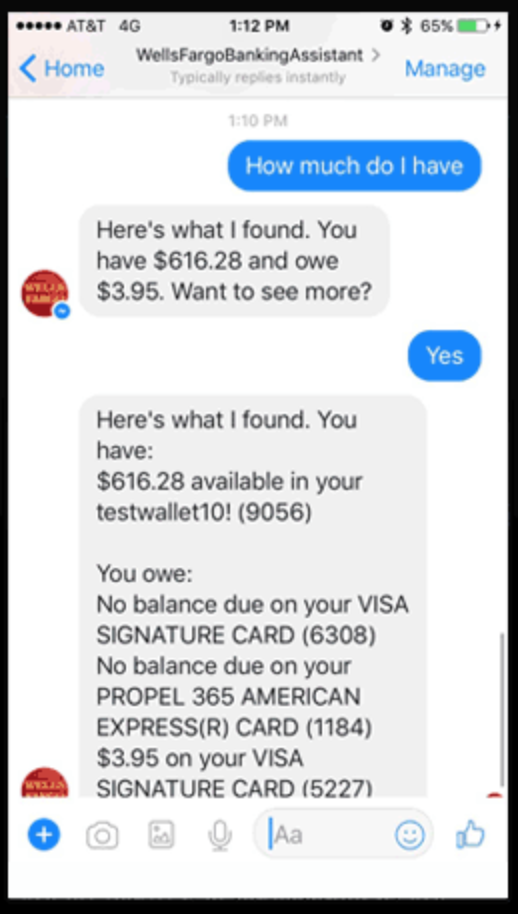
\includegraphics[width=0.3\textwidth, keepaspectratio]{images/wells_fargo_bot_1.png}
    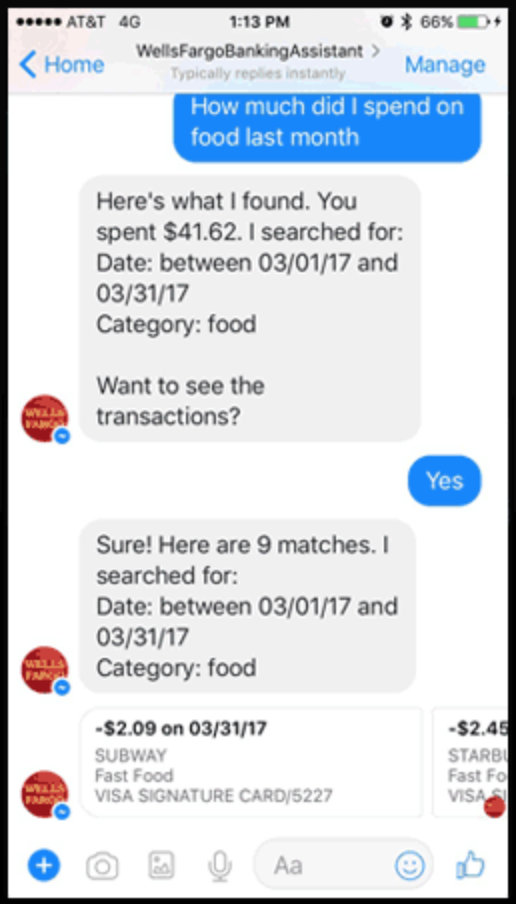
\includegraphics[width=0.3\textwidth, keepaspectratio]{images/wells_fargo_bot_2.png}
    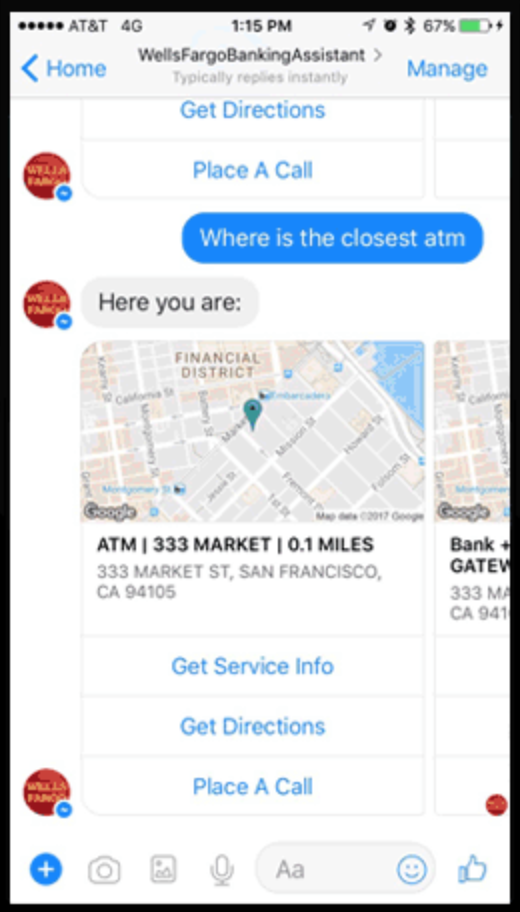
\includegraphics[width=0.3\textwidth, keepaspectratio]{images/wells_fargo_bot_3.png}
    \caption{Frontend of a Bank Assistant chat-bot by Wells Fargo on a Facebook}
    \medskip
    \footnotesize\textit{Source:} Own study
\end{figure}

Overwhelmingly, as a frontend, chatbots use textual dialog messenger and usually are associated with this form.
In this use-case customer write via suitable messenger, social network or application in an extremelly familiar environment.
Obviously, familiarity is also connected to prior existance of customer support dialogs in any form.
Nonetheless, as it was mentioned before, this is only a form of interaction, not a logic by itself and not the most labor-intensive part of the chatbot.


\subsection{Middleware}

Input received from frontend is passed to middleware.
Middleware can be either on a bank side, or on some third-party service.
Middleware is required for preprocesing of an input for processing on a bank side, or for postprocessing of an output received from a bank side for proper customer understanding.
In other words, this is a part of logic not connected to banking operations, but is required for proper understanding on both sides of interaction.

The most simple case is for Rule-based decision-making.
For this option there is no need to use complicated Statistics and Machine Learning knowledge, but input is represented by limited set of options and output is presented as a filled template answer.
This case is preferred for faster chat-bot development, or for a chat-bot on an employee side, which is hidden from a client. 

Nevertheless, middleware can have a much more complicated form.
Ideally, this is the first frontier of Artificial Intelligence and Machine Learning technics in chatbots
However, it is not used for analytics, but mainly for Natural Language Processing.

Natural Language Processing, NLP, divides in two parts — Natural Language Understanding and Natural Language Generation.
Natural Language Understanding is a branch of NLP which uses Artificial Intelligence, mostly Machine Learning technics, for building software to understand input in the form of sentences using text or speech.
Natural Language Generation is a branch of NLP which uses Artificial Intelligence, mostly Machine Learning technics, for building software to generate text and synthesize tet.

Accordingly, Conversational Banking has to be created with two instruments, Natural Language Understanding for input and Natural Language Generation for output.
Moreover, same middleware can be used for various forms, as a text or speech understanding framework for call-center bots, website chatbots or roboadvisers and for text or speech generation for SMS, text answers or cold calling.
 

\subsection{Backend}

Backend part of any conversational interaction is the most important from a banking side, as it is directly connected to banking processes.
This part is actual part of execution of transactions, request or for other orders of operations, including current balance check.
Moreover, it is inextricably linked with actual bank as a platform for financial services.
In comparison to frontend, interface for bank interaction has to be strictly formulated and defined, as, basically, this represents API, application programming interface, of a bank.

The most intense usage of AI is possible here and can be shared with all levels of banking.
The root source of data for decision-making based on AI is a metadata collected from requests.
As those request interface is strictly formulated, it is possible to define which type of data to collect, obviously, confirmed to GDPR regulations and requirements, and after proper anonymizing of corresponding data.
Backend of a chatbot should be connected to general recommendation system of a bank, as conversational banking, from a bank perspective, is yet another channel for client interaction.
Obviously, mentioned recommendation system is a main source of Machine Learning based decision-making, as it can build unpredictable models of client behaviour, both individual and as a group, and based on those models observe future client trends, give recommendations and what is even more important, contact with a client based on a made decision.

Secondly, this is a place for AI to learn customer related questions not connected to bank services, but to regulations.
For example, using supervised learning AI can learn, based on previous answers by a contact center, what documents client need to open current account or be informed about entire process of opening brokerage account.


\subsection{Conclusion}

Chatbots are an extremelly form of client interaction.
Even though latest achievements of Artificial Intelligence can and has to be applied to banking, those can be comparingly independent and developed separately and parallelly by different parties.
Moreover, those parts can be connected to existing banking services and interfaces and don't require changes other, than those required by modern banking regulations or Open Banking philosophy.
Banks can use same chatbot communication channel for notifications to increase level of client engagement.
In general, live chat can be used as a direct client communication channel with clients, provide information on product specs and services, contact info, payments proceeding, financial recommendations and many other goods and services.

It is possible to highlight several trends, which may have the most significant impact on the development of the chatbot industry in the near future.
Firstly, growth of share of combined solutions, in which robots are not able to replace human completely, but complement for repeating routine activities.
The most promising among of them are assistants for human operators, that are integrated with Robotic Process Automation.
The second trend is the development of tools for business intelligence data mining and building ontologies for unstructured data.
In other words, those are the systems into which it is possible to upload a variety of texts, and it will automatically
extract semantic connections and build language models, specific for that certain domain.
Lastly, shareable knowledge between different chatbots and chatbot platforms.
That would allow creating personified virtual assistants, with the special “personality” for each client.
As a result, we can say that Artificial Intelligence and Machine Learning mostly are being used by Front Office in a hidden for an ordinary man.

% !TeX root = ../../master_thesis.tex

\section{Strategy of a chatbot solution}

Developing a chatbot for a financial institution is expected to bring high costs and consume lots of time.
However, consequent approach to chatbot development will lead to iterative process and precise control over development of new form of client interaction.
Existing market situation already requires certain mechanism, that are required for Conversational Banking.
In Europe PSD2 made a major influence by forcing banks to make public APIs for payments and accounts.
Even though it required a lot of work, things done may become a foundation for a global Bank-as-a-Service wave of popularity.
Besides, iterative approach with proper strategy would lead to adaptation to current trends and forecast future trends.

Nowadays, Open Banking is one of the most important innovations in banking.
Moreover, the latest requirements of Bank Regulators all over the world demand this innovation. 
Thus, granting access to more banking activities and services is an obvious trend.

Currently, PSD2 demand only a small subset of operation, initiation of payments and account check.
However, this had already forced banks to know how to make secured public APIs according to regulations.
As a set of possible operation using third-party providers is limited, we can assure that there are two APIs, for internal usage and for public usage.

\mttable
{Current route of a user request to a bank}
{Own study}
{
    \begin{tikzpicture}[auto, node distance=2cm,>=latex']
        \node [block](user){User of services};
        \node [block, right = 4cm of user, above of = user](internet_banking){Internet or mobile banking};
        \node [block, right = 4cm of user, below of = user](tpp){Third-party service providers};
        \node [block, right = 1cm of internet_banking](internal_api){Internal API of a Bank};
        \node [block, right = 1cm of tpp](public_api){Public API of a Bank};

        
        \draw [->] (user) -- (internet_banking);
        \draw [->] (user) -- (tpp);

        \draw [->] (internet_banking) -- (internal_api);
        \draw [->] (internet_banking) -- (public_api);
        \draw [->] (tpp) -- (public_api);
    \end{tikzpicture}
}

Accordingly, internal bank API is used for official bank's internet banking web application or mobile banking application. 
Obviously, same internal API can be used for internal usage among internal bank services.
More or less, mentioned graph represents current state of banking interaction with third-party services from a client side.


\subsection{Open Banking API development and extension}

In ideal world it would be easy and comfortable for banks to make entire API public and supportable.
This would allow banks to focus on financial operations and stability, instead of front-offices.
Unfortunately, this is not possible due to tactical reasons and obvious risks for such major changes.
Nevertheless, we can assume that certain forms of financial services can be used via public API.

API is a programming interface from a set of ready-made functions or structures that are provided by an application or service.
This API has to support as many banking services, as possible, both for registered, bank, users and newcomers. 
Among those services could be, among PSD2-based balance check and setting payments, as listing public or individual offers, loan requirements check, deposit terms, additional services and legal information.

As a second step, banks have to make mentioned API public or licensable.
Basically, this would allow for bank to work in a Bank-as-a-Service business model in a more abstract way.
The reasoning behind this is in high costs of internal solutions. 
Additionally, bank may not be interested or cannot allow for itself to invest into risky forms of client interaction.
Bank-as-a-Service model for third-party FinTechs is an applicable option in this case, as it would allow transferring customer interaction risks to FinTechs.
This is the very first step where AI is usable in any form.
Basically, this step represents risk deduction by allowing FinTech using Bank-as-a-Service.
How to create client interaction, how to analyze client interaction and how to interpret results becomes a problem for third-parties.

In this case, bank can check and validate strategies done by third-parties for client interaction, and in case of positive impact bank can decide what is more applicable — either to continue serving as a service bank, or to create new ways of client interaction by itself.

\mttable
{Open Banking User Request Route}
{Own study}
{
    \begin{tikzpicture}[auto, node distance=2cm,>=latex']
        \node [block](user){User of services};
        \node [block, right = 5cm of user, above of = user](internet_banking){Internet or mobile banking};
        \node [block, right = 5cm of user, below of = user](tpp){Third-party service providers};
        \node [block, right = 5cm of tpp, above of = tpp](api){Public API of a Bank};

        
        \draw [->] (user) -- (internet_banking);
        \draw [->] (user) -- (tpp);

        \draw [->] (internet_banking) -- (api);
        \draw [->] (tpp) -- (api);
    \end{tikzpicture}
}

This development would lead to a major move towards Bank-as-a-Service.
Allowing third-party providers to use bank's own services via API on defined and specified requirements would lead to partly delegation of front-office functions to those third-parties, as those can focus on B2C cooperation and find clients more precisely and in more effective way, especially by uniting services of multiple Banks-as-a-Services.
Mentioned operations would inevitably result in risky, state-of-art FinTech start-ups.
As a result, Conversational Banking solution can be created by a FinTech start-up, resulting in a next operational scheme.

\mttable
{Open Banking User Request Route with Conversational Banking}
{Own study}
{
    \begin{tikzpicture}[auto, node distance=2cm,>=latex']
        \node [block](user){User of services};

        \node [block, right = 1cm of user](tpcb){Third-party conversational banking};
        \node [block, above of = tpcb](internet_banking){Internet or mobile banking};
        \node [block, below of = tpcb](tpp){Third-party service providers};
        
        \node [block, right = 1cm of tpcb](api){Public API of a Bank};

        
        \draw [->] (user) -- (internet_banking);
        \draw [->] (user) -- (tpcb);
        \draw [->] (user) -- (tpp);

        \draw [->] (internet_banking) -- (api);
        \draw [->] (tpcb) -- (api);
        \draw [->] (tpp) -- (api);
    \end{tikzpicture}
}

Even though it looks like innovation, actually this is an evolution.
If bank decide to turn to Conversational Banking in all cases it has to create secure API for multiple operations not covered by, for example, PSD2 yet.
It is a wise option to share API for third-party service providers, as it would allow testing innovations by costs of third-party providers.


\subsection{Rule-based middleware}

Undoubtedly, bank should not rely only on third-parties, but has to create own solutions.
Firstly, bank has to create comparably simple and low-cost middleware for a chatbot.
Of course, this is not an Artificial Intelligence, as it may require big investments, but a more simple, rule-based algorithmic solution.
Unfortunately, in both cases additional costs are required on a front-end level, either some user interface changes in mobile and internet banking application, as a chat window for bot is required.
On the other hand, an additional application for front-office employees is required, if banks decide to make a hybrid chatbot approach.

\mttable
{User Request Route with Rule-based middleware}
{Own study}
{
    \begin{tikzpicture}[auto, node distance=2cm,>=latex']
        \node [block](rbm){Rule-based middleware};
        
        \node [block, above of = rbm, left of = rbm](user){User of services};
        \node [block, below of = rbm, left of = rbm](employee){Front-office employee};
        
        \node [block, right = 1cm of rbm](capi){Conversational API of a Bank};
        \node [block, above of = capi](papi){Public API of a Bank};
        \node [block, below of = capi](kdb){Knowledge database};

        \draw [->] (user) -- (rbm);
        \draw [->] (employee) -- (rbm);
        \draw [->] (rbm) -- (capi);
        \draw [->] (capi) -- (papi);
        \draw [->] (capi) -- (kdb);
    \end{tikzpicture}
}

Additional costs are required on a back-end side for a Conversational API, which should handle requests from middleware and return formed responses.
As well, Conversational API has to use knowledge database, which has predefined answers for most popular questions or some templates.


\subsection{Middleware with Machine Learning}

The most ambitious, innovative and risky form of a chatbot would be a chatbot which uses Artificial Intelligence, Machine Learning and Natural Language Processing techniques for client communication.
Entire processing would be done on a middleware between a user interface, which is used either by a client or an employee, and a bank's back-end API.

Machine Learning based middleware, either third-party or owned and developed by bank, processes human-written text to a form of a back-end request and generates human-readable answer based on a response received from a bank back-end.

\mttable
{Open Banking User Request Route with ML\&AI Conversational Banking}
{Own study}
{
    \scalebox{0.9}{
        \begin{tikzpicture}[auto, node distance=2cm,>=latex']
            \node [block](employee){Front-office employee};
            \node [block, below = 3cm of employee](user){User of services};
            
            \node [block, right = 1cm of employee, align = center](bmml){Bank's middleware with ML\&AI};
            \node [block, right = 1cm of user, below = 3cm of bmml](tpmml){Third-party middleware with ML\&AI};
            
            \node [block, right = 6cm of bmml, below of = bmml](capi){Conversational API of a Bank};
            
            \node [block, above of = capi](papi){Public API of a Bank};
            \node [block, below of = capi](kdb){Knowledge database};

            \draw [->] (employee) -- (bmml);
            
            \draw [->] (user) -- (bmml);
            \draw [->] (user) -- (tpmml);
            
            \draw [->] (bmml) -- (capi);
            \draw [->] (tpmml) -- (capi);
            
            \draw [->] (capi) -- (papi);
            \draw [->] (capi) -- (kdb);
        \end{tikzpicture}
    }
}

Basically, an ideal system should be just an intermediate block of logic, that receives message from a client, determines business related data and transfers it to customer relationship management system.
Accordingly, CRM system returns data, which is used by a mentioned block of logic, which returns human-readable format.
Of course, it has to use various databases of known question-answer pairs and lists of promoted products.

\mttable
{Structure of an integrated chatbot solution}
{Own study}
{
    \begin{tikzpicture}[auto, node distance=2cm,>=latex']
        \node [block]
            (user){User};
        \node [block, right of = user, node distance = 4cm]
            (bot){Chatbot};
        \node [block, right of = bot, node distance = 4cm]
            (output){CRM};
        \node [block, below of = bot, node distance = 2.5cm]
            (database){Database};
        \draw [<->] (user) -- (bot);
        \draw [<->] (bot) -- (output);
        \draw [<->] (bot) -- (database);
        \draw [<->] (database) -| (output);
    \end{tikzpicture}
}

Unfortunately, this type of system would be significantly complicated and requires more precise analysis and planning.
Firstly, a user-input message has to pass data cleansing and go to NLU engine, which transforms a message into contextual keywords, which would allow dialog manager to handle.
More simple forms, which can be templated or is a common knowledge, for example, currency rates, can be received via database of questions and answers.
More complicated logic has to be handled in Dialog Manager.
As a result, formed response passes to NLG engine, which generates text or synthesizes speech, which is passed as an output to user.
Obviously, for development reasons dialog has to be collected and analyzed with metadata. 
Accordingly, Artificial Intelligence is a main logical solution for Natural Language Understanding, Natural Language Generation, Dialog Manager and Analytics.

\begin{sidewaystable}
    \caption{Structure of a ML\&AI chatbot solution with Natural Language Processing}
    \begin{center}
    \begin{tikzpicture}[auto, node distance=4cm,>=latex']
        \node [block](messenger){Messenger};
        \node [block, right of = messenger]
            (cleansing){Data cleansing};
        \node [block, right of = cleansing, align = center]
            (nlu){Nature\\ Language\\ Understanding\\ (NLU)};
        \node [block, right of = nlu, below of = nlu, align = center]
            (dm){Dialog Manager\\ (DM)};
        \node [block, right of = nlu, above of = dm]
            (dlog){Dialog log};
        \node [block, right of = dlog]
            (analytics){Analytics};
        \node [block, below of = dm, align = center]
            (base_database){Database of\\ questions and answers};
        \node [block, below of = cleansing, align = center]
            (nlg){Nature\\ Language\\ Generator\\ (NLG)};
        \draw [->] (messenger) -- node{$Input$} (cleansing);
        \draw [->] (cleansing) -- (nlu);
        \draw [->] (nlu) -| node[align = center]{$Keywords$} (dm);
        \draw [->] (dm) -| (dlog);
        \draw [->] (dlog) -- (analytics);
        \draw [<->] (dm) -- (base_database);
        \draw [->] (dm) -- node{$Next$ $question$} (nlg);
        \draw [->] (nlg) -| node{$Output$} (messenger);
    \end{tikzpicture}
    \end{center}
    \medskip
    \source{Own study}
\end{sidewaystable}

\subsection{Recommendations and notifications}

However, AI in a chatbot is not limited to practical use in terms of Natural Language Processing.
AI can be used to create powerful recommendation and notification system, based on existing categories of users and their preferences.

\mttable
{Plan of integration of a ML\&AI Recommendation and Notification systems}
{Own study}
{
    \begin{tikzpicture}[auto, node distance=2cm and 1cm,>=latex']
        \node [block](capi){Conversational API of a Bank};
        \node [block, above of = capi](papi){Public API of a Bank};
        \node [block, below of = capi](kdb){Knowledge database};

        \node [block, right = of capi](m_and_a){Analytics engine};

        \node [block, right = of m_and_a](recs){ML\&AI Recommendations};
        \node [block, below = of recs](nots){Notifications};

        \draw [->] (capi) -- (papi);
        \draw [->] (capi) -- (kdb);
        \draw [->] (capi) -- (m_and_a);
        \draw [->] (m_and_a) -- (recs);
        \draw [->] (recs) -- (nots);
    \end{tikzpicture}
}

Every request received may have meta-information, as popular keywords, popular requests, which in pair with known customer information, as age, location, gender and other, allows bank to build recommendation system based on a Machine Learning solutions.
Nonetheless, this can be done both on a bank side, as on third-party solution, resulting in a Bank-as-a-Platform form of development in this case.

Obviously, generated recommendations should be somehow delivered to a user.
This can be done not only by a common form of web, mobile or SMS notifications, but also in a form of a message via same chatbot, which is an important form of communication initiation from a bank's side in case of chatbots in social networks and third-party messengers.

\subsection{Summary of approaches}

Every stage can be done in 3 possible ways:
\begin{enumerate}
    \item Software-as-a-Service
    \item Solution on premise
    \item In-house development
\end{enumerate}

The cheapest and fastest way would be to use Software-as-a-Service solution, which has minimal technical requirements, requires minimal maintenance and just has to be integrated into bank's infrastructure. 
On the other hand, usually there is no possibility to customize mentioned solution and requires additional vendor support. 
Moreover, finding a proper vendor is a complicated task, as a vendor has to have banking experience and proof-of-work.

As an option, bank can interact with a vendor to create solution on premise. 
In this case it would be entirely controllable and suited to bank's needs. 
Contrarily, it would require much more resources for both integration process and support.

The most precise and leading option for every bank would be to create own in-house solution, which would, obviously, give bank entire control over both support, costs, efficiency and services supported.
Nevertheless, this is the most expensive solution both in costs and time consumption, as it would not only require to build additional divisions both for development and maintenance, but also requires in-depth understanding of various technical and security standards.
According to studies, implementation costs time consumption of PSD2 varied drastically based on a chosen way of development and size of a bank. 
\cite{saltedge_open_banking_report}
\cite{deloitte_psd2_costs}

\mttable
{Average costs of PSD2 implementation}
{Own study, based on "European PSD2 Survey Results highlights", Deloitte, 2017, p.5.}
{
    \begin{tabular}{| c | c | c | c |}
        \hline
        &
        \textbf{Development costs, \$} & 
        \textbf{Annual fees, \$} &
        \textbf{Time, months} \\ \hline 
       
        \textbf{Software-as-a-Service} & 
            15'000-30'000 & 
            30'000-300'000 &
            1-3 \\ \hline 
       
        \textbf{Solution on premise} & 
            500'000 &
            100'000 &
            6-18 \\ \hline 

        \textbf{In-house development} &
            200'000-1'000'000 &
            50'000-200'000 &
            12-24 \\ \hline
    \end{tabular}
}

As it was mentioned before, public API is a wider approach, which is based on infrastructure and system provided during implementation of PSD2.
As a result, in my opinion it is possible to apply same expectations to development of public API.

\mttable
{Expected costs of an Open Banking API implementation}
{Own study}
{
    \begin{tabular}{| c | c | c | c |}
        \hline
        &
        \textbf{Development costs, \$} & 
        \textbf{Annual fees, \$} &
        \textbf{Time, months} \\ \hline 
       
        \textbf{Software-as-a-Service} & 
            15'000-30'000 & 
            30'000-300'000 &
            1-3 \\ \hline 
       
        \textbf{Solution on premise} & 
            500'000+ &
            100'000+ &
            6-18 \\ \hline 
            
        \textbf{In-house development} &
            200'000-1'000'000 &
            50'000-200'000 &
            12-24 \\ \hline
    \end{tabular}
}

The next step is to build a cheaper version of middleware, rule-based.
What is even more important, in case of having sufficient budget, this solution can be done in parallel with API extension and UI of front-office development.
Therefore, time to market for middleware highly depends on chosen strategy and available budget.

\mttable
{Expected costs of a Rule-based middleware solution}
{Own study}
{
    \begin{tabular}{| c | c | c | c |}
        \hline
        &
        \textbf{Development costs, \$} & 
        \textbf{Annual fees, \$} &
        \textbf{Time, months} \\ \hline 
       
        \textbf{Software-as-a-Service} & 
            10'000-25'000 & 
            25'000-60'000 &
            1-3 \\ \hline 
       
        \textbf{Solution on premise} & 
            50'000+ &
            50'000+ &
            4-6 \\ \hline 
            
        \textbf{In-house development} &
            100'000+ &
            50'000+ &
            4-6 \\ \hline
    \end{tabular}
}

Next logical step would be creation of Machine Learning based middleware.
This step is the most intense and the most expensive stage.
Additionally, this stage cannot be done parallelly with other stages, as it requires enormous investments and development involvement, which adversely affect time consumption.
However, it is not the only negative affect, as this stage additionally requires using supervised Machine Learning, which requires sequential time-consuming stages, as data collection, teaching process and model testing.
Nevertheless, time to market is even longer if this middleware has to be used for customer related chatbot, as, firstly, it has to be used by employees.
The best use-case would be to use hybrid chatbot approach, which allows unsupervised learning by observing dialog between employee and a client at first.
Secondly, employee would just be an additional layer between middleware and chatbot, which results in a supervised learning, where employee is the teacher.
Mentioned strategy allows developing highly efficient chatbot without need to test in production on existing users.

\mttable
{Expected costs of a ML\&AI middleware solution}
{Own study}
{
    \begin{tabular}{| c | c | c | c |}
        \hline
        &
        \textbf{Development costs, \$} & 
        \textbf{Annual fees, \$} &
        \textbf{Time, months} \\ \hline 
       
        \textbf{Software-as-a-Service} & 
            25'000-50'000 & 
            25'000-50'000 &
            4-6 \\ \hline 
       
        \textbf{Solution on premise} & 
            150'000-500'000 &
            50'000 &
            6-9 \\ \hline 
            
        \textbf{In-house development} &
            300'000-1'000'000 &
            50'000-200'000 &
            9-15 \\ \hline
    \end{tabular}
}

Machine Learning based chatbot with Natural Language Processing is an extremely efficient banking solution.
It allows supplying content and information based on a habits and requirements of a user.
Especially, it increases user engagement due to fast replies and understandable form of help.
However, chatbot by form of user interaction does not answer the questions, which user does not ask.
As a result, user cannot ask about the services he does not know about.
Moreover, this solution does not cover purposes of bank growth and development.

In order to fulfill those banking needs, additional system of recommendations and notifications is required.
This system should allow based on existing, known customer data give personalized recommendations either by form of additional answers in a chatbot, dialog initiation message or notifications.

\mttable
{Expected costs of ML\&AI-based Recommendation and Notification solution}
{Own study}
{
    \begin{tabular}{| c | c | c | c |}
        \hline
        &
        \textbf{Development costs, \$} & 
        \textbf{Annual fees, \$} &
        \textbf{Time, months} \\ \hline 
       
        \textbf{Software-as-a-Service} & 
            15'000-30'000 & 
            6'000-15'000 &
            1-3 \\ \hline 
       
        \textbf{Solution on premise} & 
            25'000-50'000 &
            10'000-25'000 &
            1-3 \\ \hline 
            
        \textbf{In-house development} &
            100'000-300'000 &
            50'000-100'000 &
            4-6 \\ \hline
    \end{tabular}
}

As a result, bank would be able to create new system, a chatbot with high levels of user engagement and a foretelling growth basis.
Existing forms of development are extremely flexible and can suit any forms of budget and time available.
Banks can choose a level of influence and control over product based on their needs.
Nonetheless, entire system and approach is a very risky form of investment and should be extremely precisely analyzed by management.

\mttable
{Expected costs of an AI NLP chatbot solution with Recommendations}
{Own study}
{
    \begin{tabular}{| c | c | c | c |}
        \hline
        &
        \textbf{Development costs, \$} & 
        \textbf{Annual fees, \$} &
        \textbf{Time, months} \\ \hline 
       
        \textbf{Software-as-a-Service} & 
            65'000-135'000 & 
            86'000-425'000 &
            6-12 \\ \hline 
       
        \textbf{Solution on premise} & 
            725'000-1'100'00 &
            210'000-300'000 &
            9-18 \\ \hline 
            
        \textbf{In-house development} &
            700'000-2'500'000 &
            200'000-550'000 &
            12-24 \\ \hline
    \end{tabular}
}

% !TeX root = ../../master_thesis.tex

\section{Research design}

As it was previously analyzed, chatbot solution may require both a lot of time and a lot of resources to develop.
Intuitively, we may expect mentioned ML\&AI-based chatbots to be an ideal, automated solution for cost decrease and effective customer support.
Unfortunately, banking clients may have subjectively negative opinion on existing rule-based chatbots, which are usually considered as an avant-garde of customer support, but may not help properly client needs.

Therefore, survey was conducted in order to determine current level of satisfaction with front-office.
In entire survey 278 respondents were involved.
The questions are as follows:

% !TeX root = ../master_thesis.tex

\annex{Survey. Satisfaction with Digital Banking Customer Service}
{\parindent0pt

1. How old are you?\par
\begin{tabular}{l c}
    18-32 & \checkbox \\
    33-48 & \checkbox \\
    49+ & \checkbox \\

\end{tabular}

\par\vspace{24pt}

2. How many banks did you interact with for the last year? \par
Number: \inputfield{24pt}

\par\vspace{24pt}

Indicate your opinion about each of the following statements.
\setlength\LTleft{-5pt}
\setlength\LTright{0pt}
\begin{longtable}{l c c c c c}
    \shortstack{}
        & \shortstack{Strongly\\Agree}
        & Agree
        & Neutral
        & Disagree
        & \shortstack{Strongly\\Disagree}
        \\

    3. I am satisfied with my banking\\\hspace{4.5mm}interactions for the last year
        & \checkbox
        & \checkbox
        & \checkbox
        & \checkbox
        & \checkbox 
        \\

    4. It was easy to solve all my problems 
        & \checkbox
        & \checkbox
        & \checkbox
        & \checkbox
        & \checkbox 
        \\

    5. I've been satisfied with response time
        & \checkbox
        & \checkbox
        & \checkbox
        & \checkbox
        & \checkbox 
        \\

    6. I prefer dialog interaction over phone calls
        & \checkbox
        & \checkbox
        & \checkbox
        & \checkbox
        & \checkbox 
        \\

    7. I can identify when I talk with a chatbot
        & \checkbox
        & \checkbox
        & \checkbox
        & \checkbox
        & \checkbox 
        \\

    8. I am satisfied with chatbots
        & \checkbox
        & \checkbox
        & \checkbox
        & \checkbox
        & \checkbox 
        \\

    9. I trust humans more than chatbots
        & \checkbox
        & \checkbox
        & \checkbox
        & \checkbox
        & \checkbox 
        \\

\end{longtable}
}


First question was to build an age portrait. 
Age answers were divided in three categories based on generation experience with dialog interfaces.
First group lower limit of 18 years was chosen due to socially acceptable age of responsibility.
First group upper limit of 32 years was chosen as dialog interfaces became most viable nearly 15 years ago, resulting in experienced users of dialog interfaces.
Second group upper limit was chosen based on a socially acceptable middle-age medium. 
It is possible to observe dominance of young generation among respondents.

\mtfigure[p]
{Ages of respondents}
{Own study}
{
    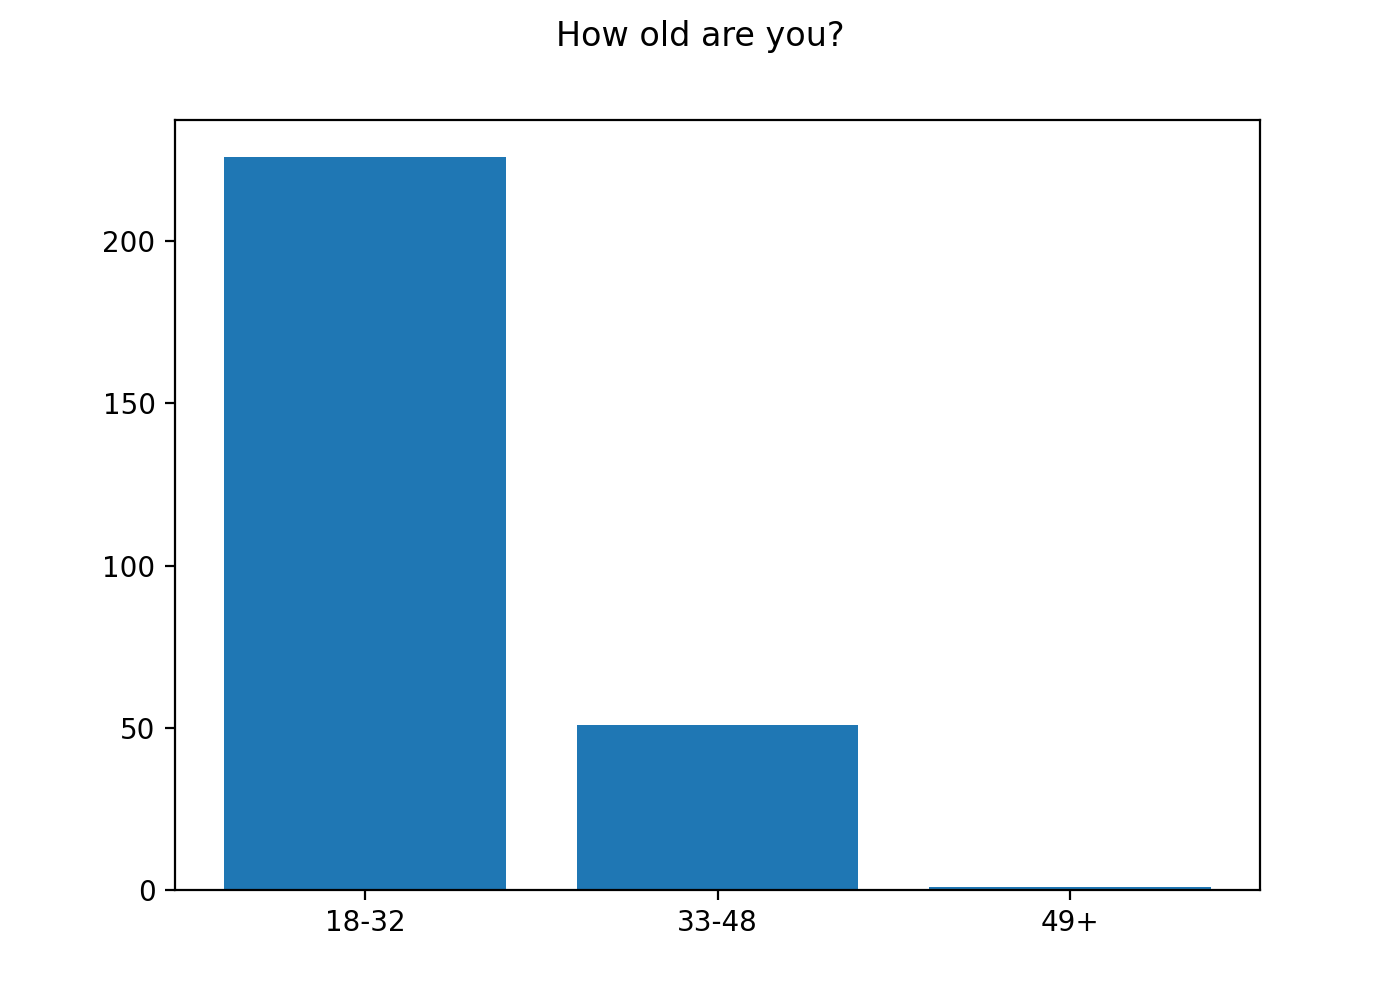
\includegraphics[width=0.6\textwidth,height=\textheight,keepaspectratio]{survey/1_how_old_are_you.png}
}

On the other hand, second question had shown high levels experience of banking interactions among respondents, as more than a half of respondents used services of 2 or more banks for the last year.

\mtfigure
{Number of banks per respondent}
{Own study}
{
    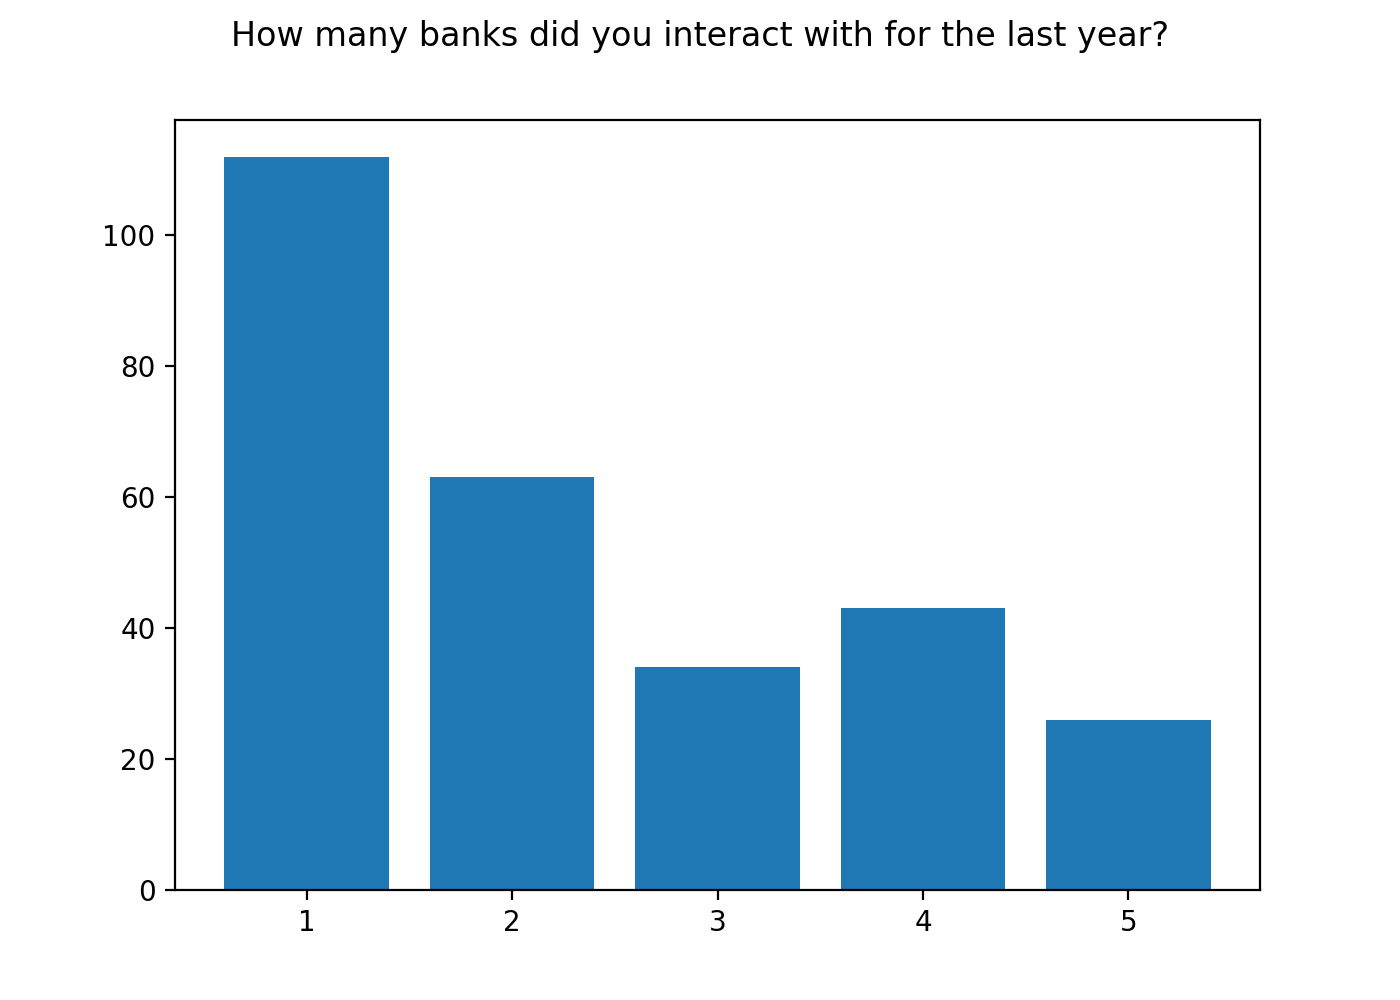
\includegraphics[width=0.6\textwidth,height=\textheight,keepaspectratio]{survey/2_how_many_banks_did_you_interact_with_for_the_last_year.png}
}

However, next two questions, question about satisfaction with banking interactions and question about satisfaction with problem-solving, had shown slightly negative feeling towards existing customer support systems.

\mtfigure
{Satisfaction with banking interaction}
{Own study}
{
    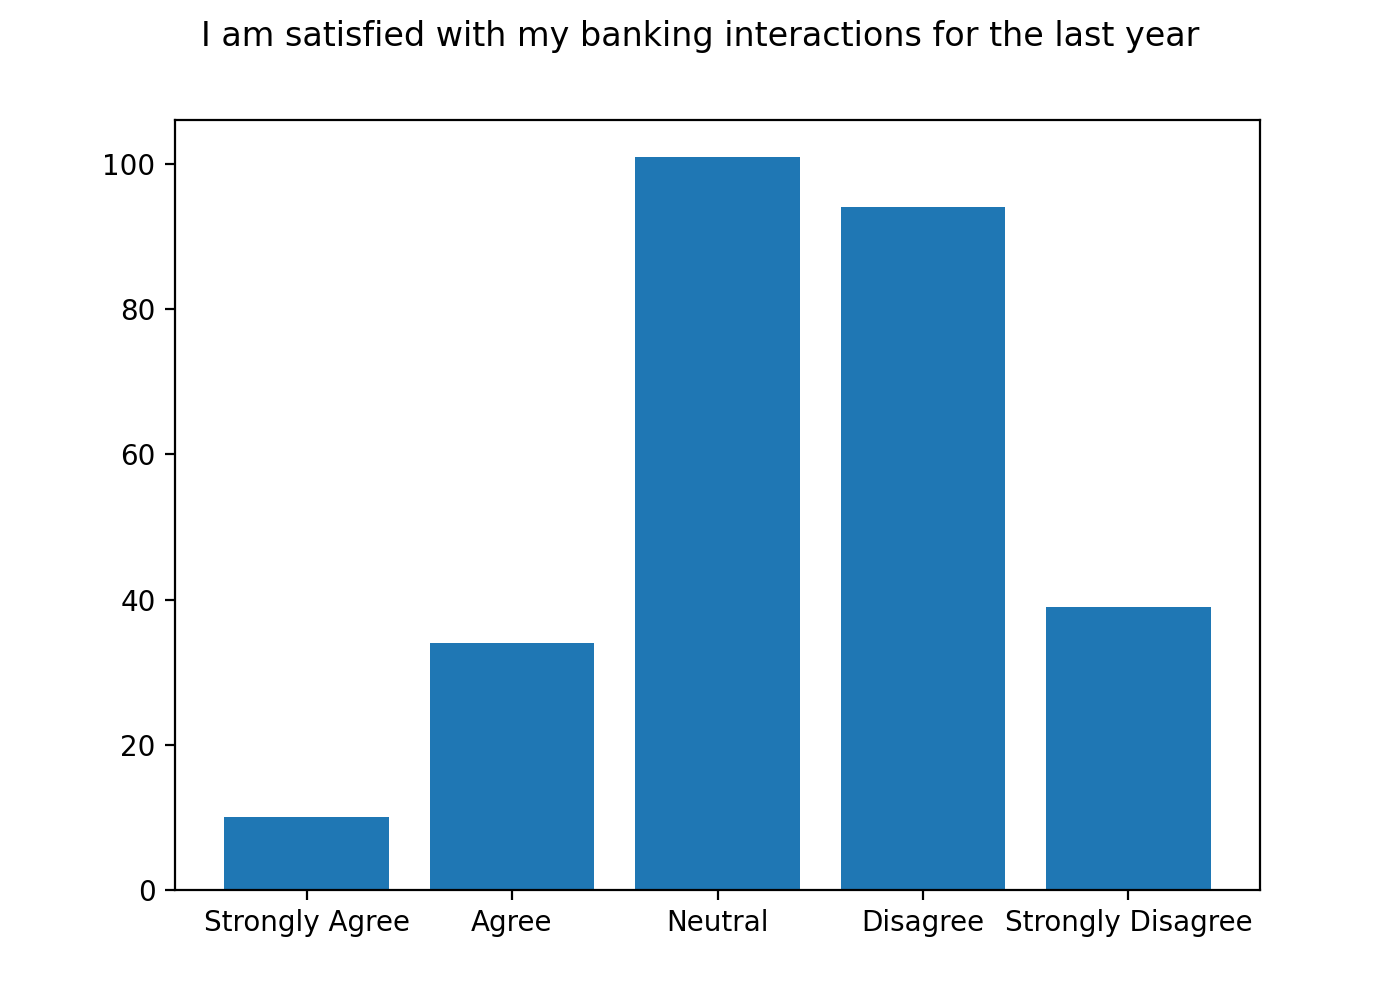
\includegraphics[width=0.6\textwidth,height=\textheight,keepaspectratio]{survey/3_i_am_satisfied_with_my_banking_interactions_for_the_last_year.png}
}

\mtfigure
{Satisfaction with problem-solving}
{Own study}
{
    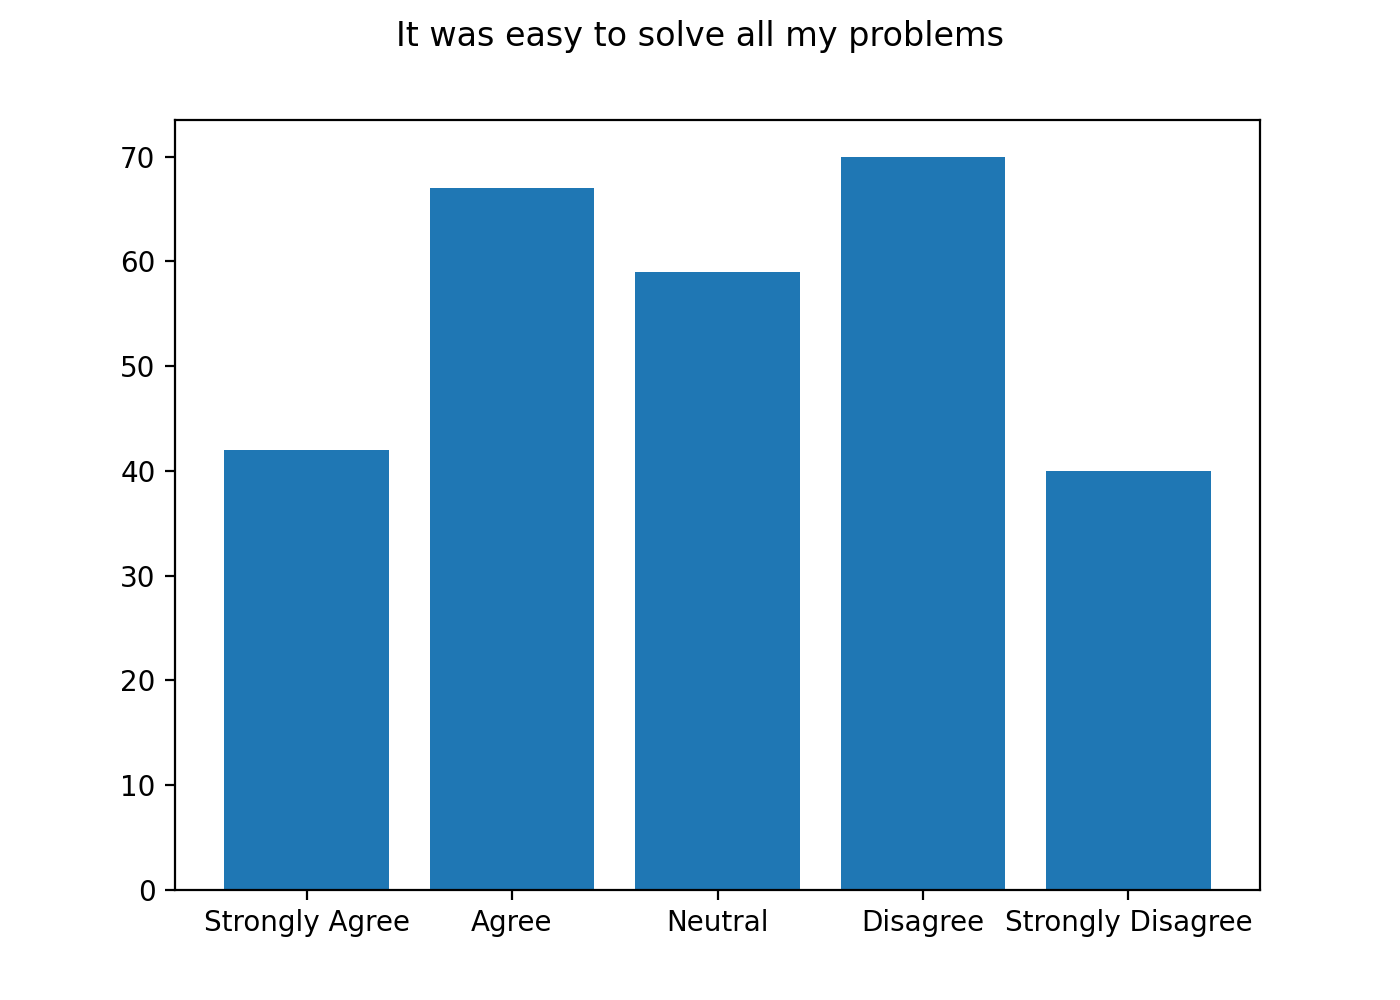
\includegraphics[width=0.6\textwidth,height=\textheight,keepaspectratio]{survey/4_it_was_easy_to_solve_all_my_problems.png}
}

At the same time, even though most of the researches had shown general dissatisfaction with response times, respondents of this survey were more loyal and showed neutrality.

\mtfigure
{Satisfaction with response time}
{Own study}
{
    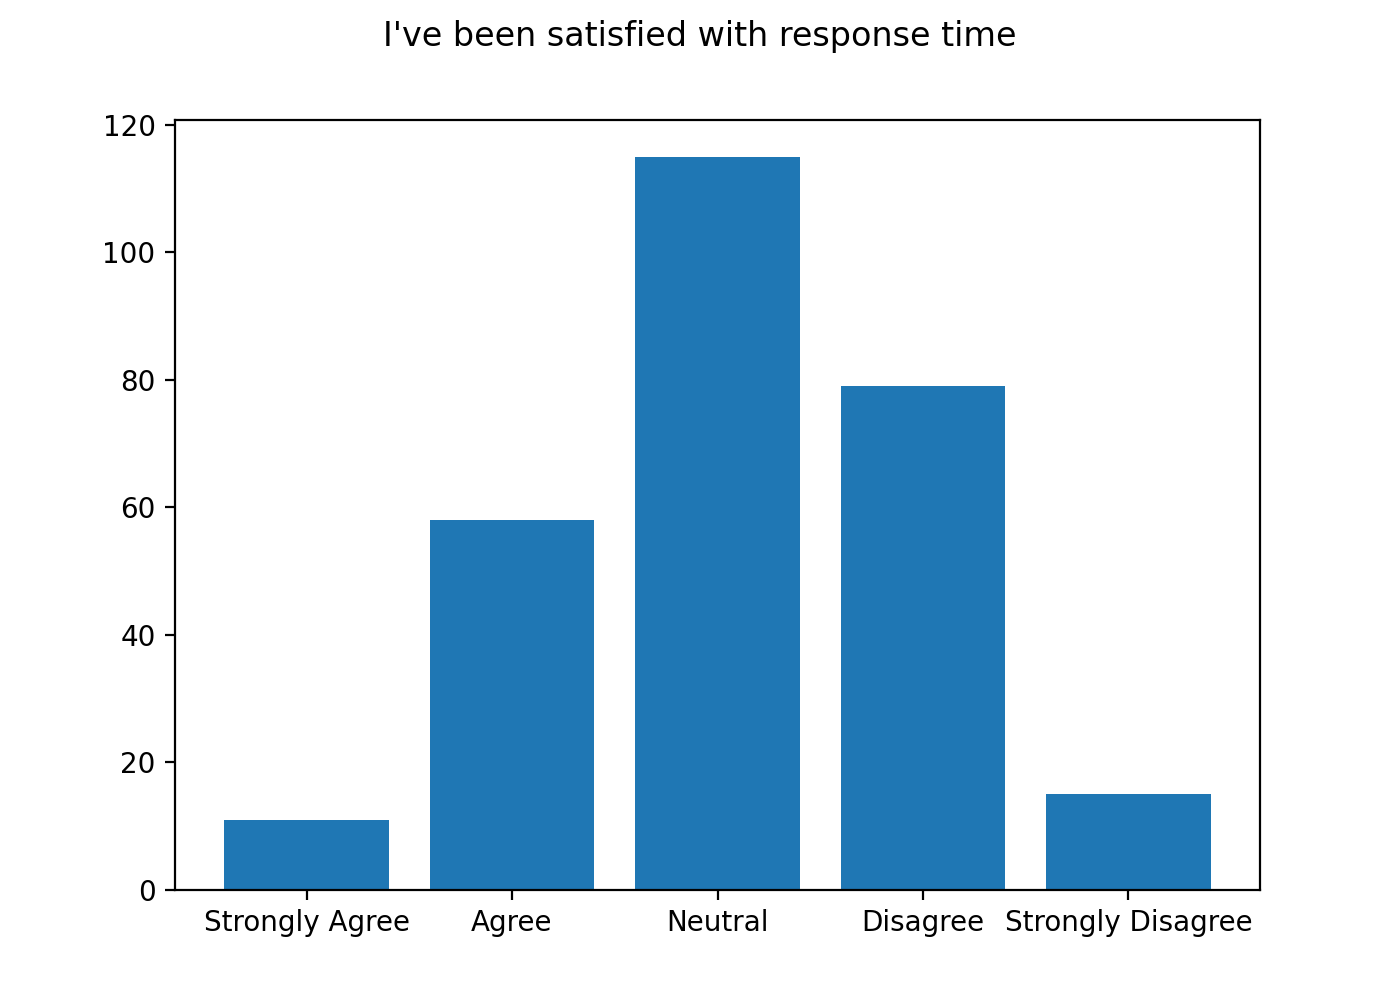
\includegraphics[width=0.6\textwidth,height=\textheight,keepaspectratio]{survey/5_i've_been_satisfied_with_response_time.png}
}

Next question confirmed hypothesis about survey population and showed that respondents mostly prefer dialog interactions over phone calls.

\mtfigure
{Preferences between dialog and calls}
{Own study}
{
    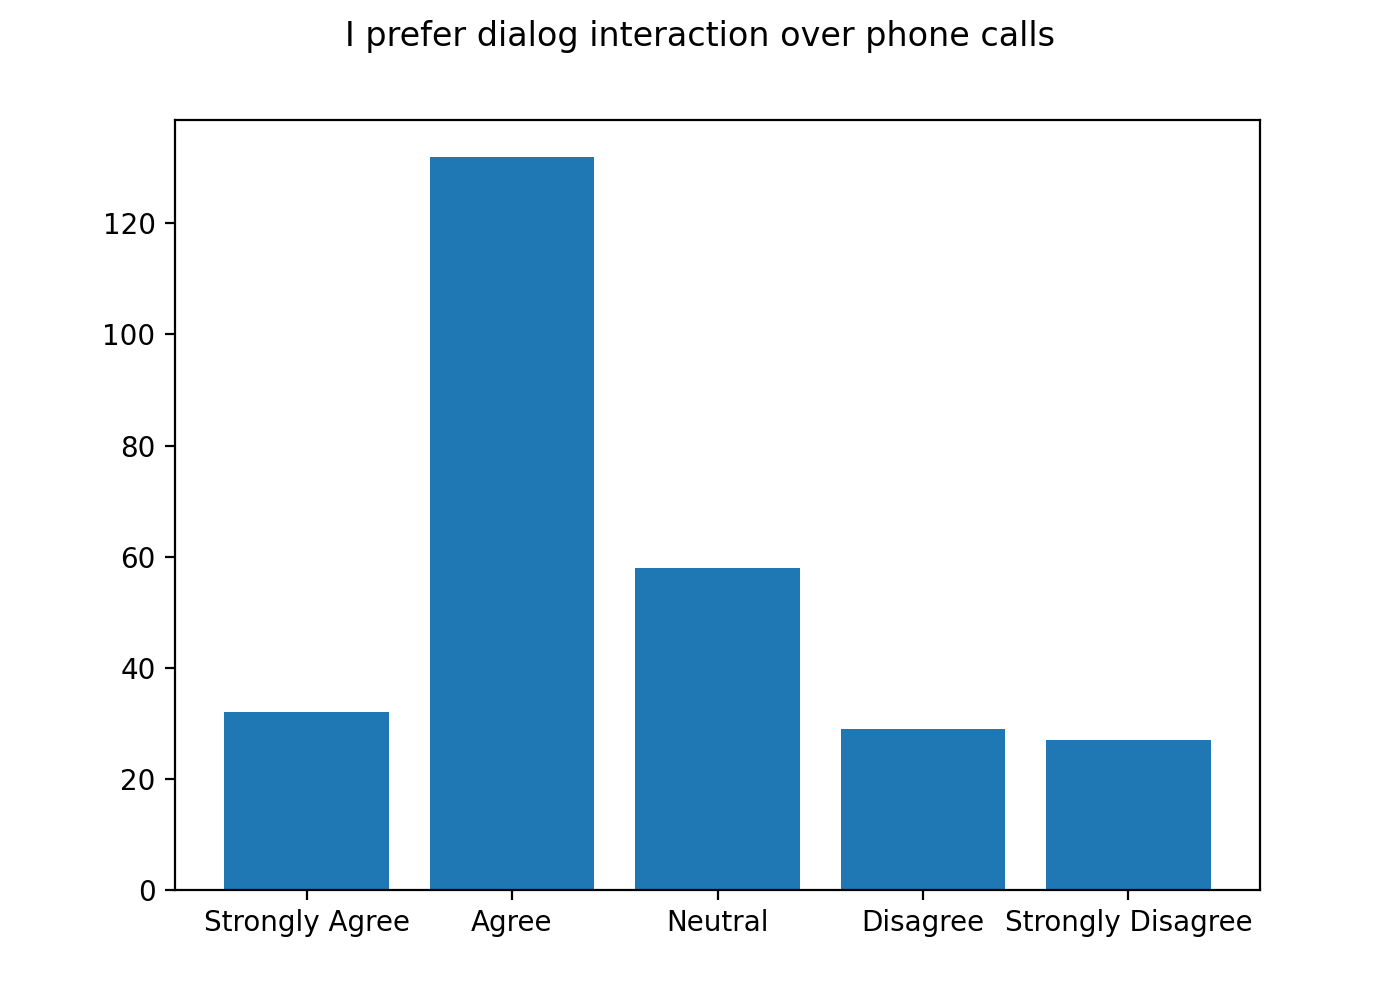
\includegraphics[width=0.6\textwidth,height=\textheight,keepaspectratio]{survey/6_i_prefer_dialog_interaction_over_phone_calls.png}
}


\subsection{Research Population and Data Collection}

One of the most interesting results is high assurance of respondents that they know when they walk with a chatbot, and not a human employee.

\mtfigure
{Chatbot awareness}
{Own study}
{
    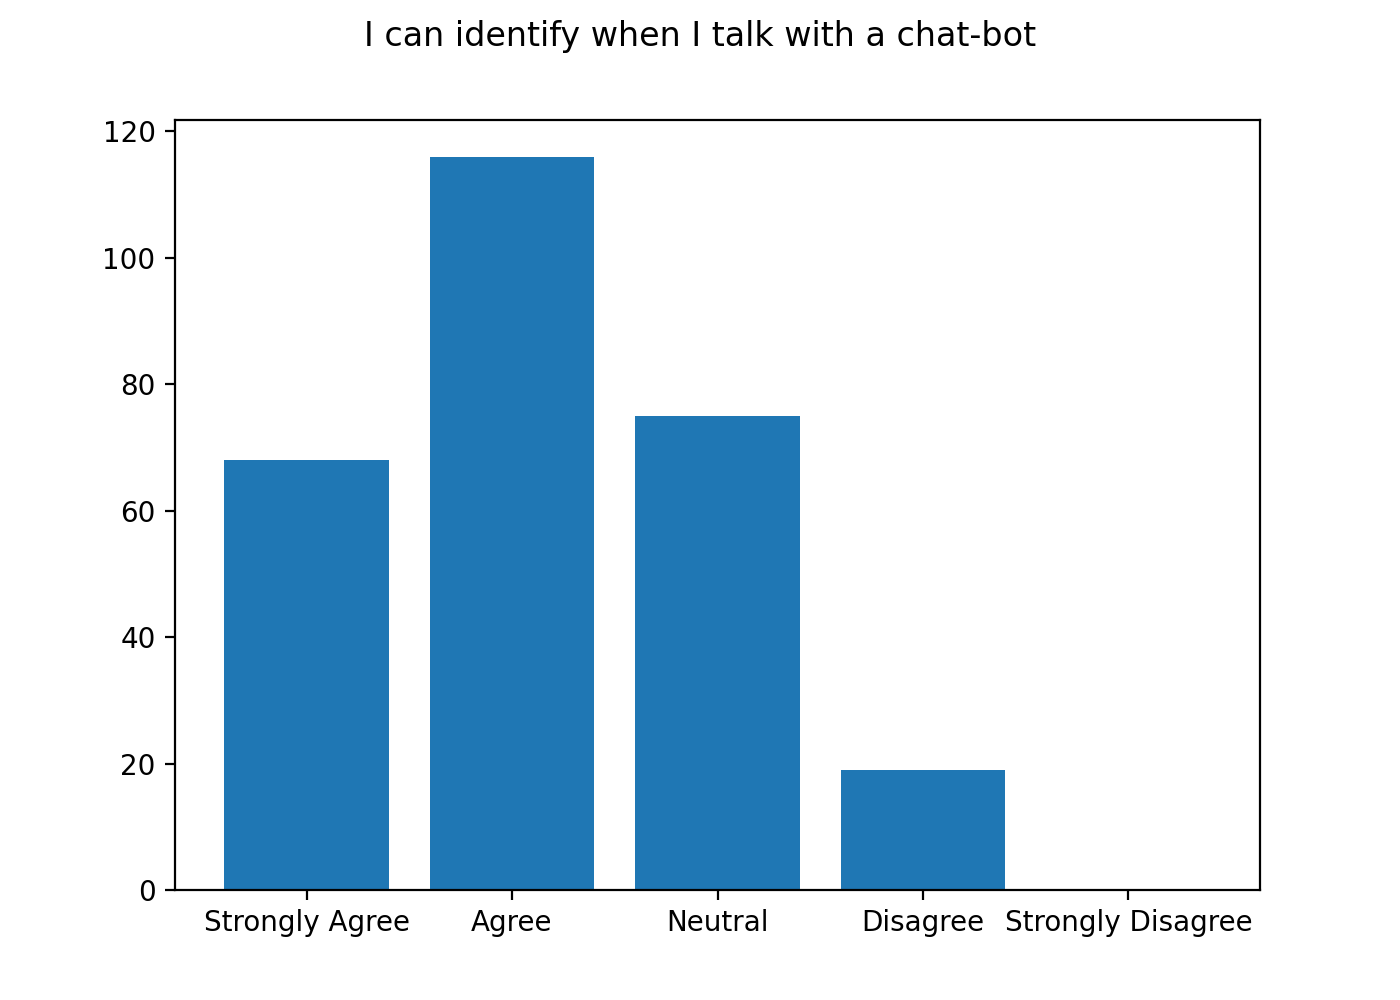
\includegraphics[width=0.6\textwidth,height=\textheight,keepaspectratio]{survey/7_i_can_identify_when_i_talk_with_a_chat-bot.png}
}

However, I suspect this is connected to significant dissatisfaction with chatbots, as there is a perfect negative correlation between questions about chatbot awareness and satisfaction with chatbots.

\mtfigure
{Satisfaction with chatbot}
{Own study}
{
    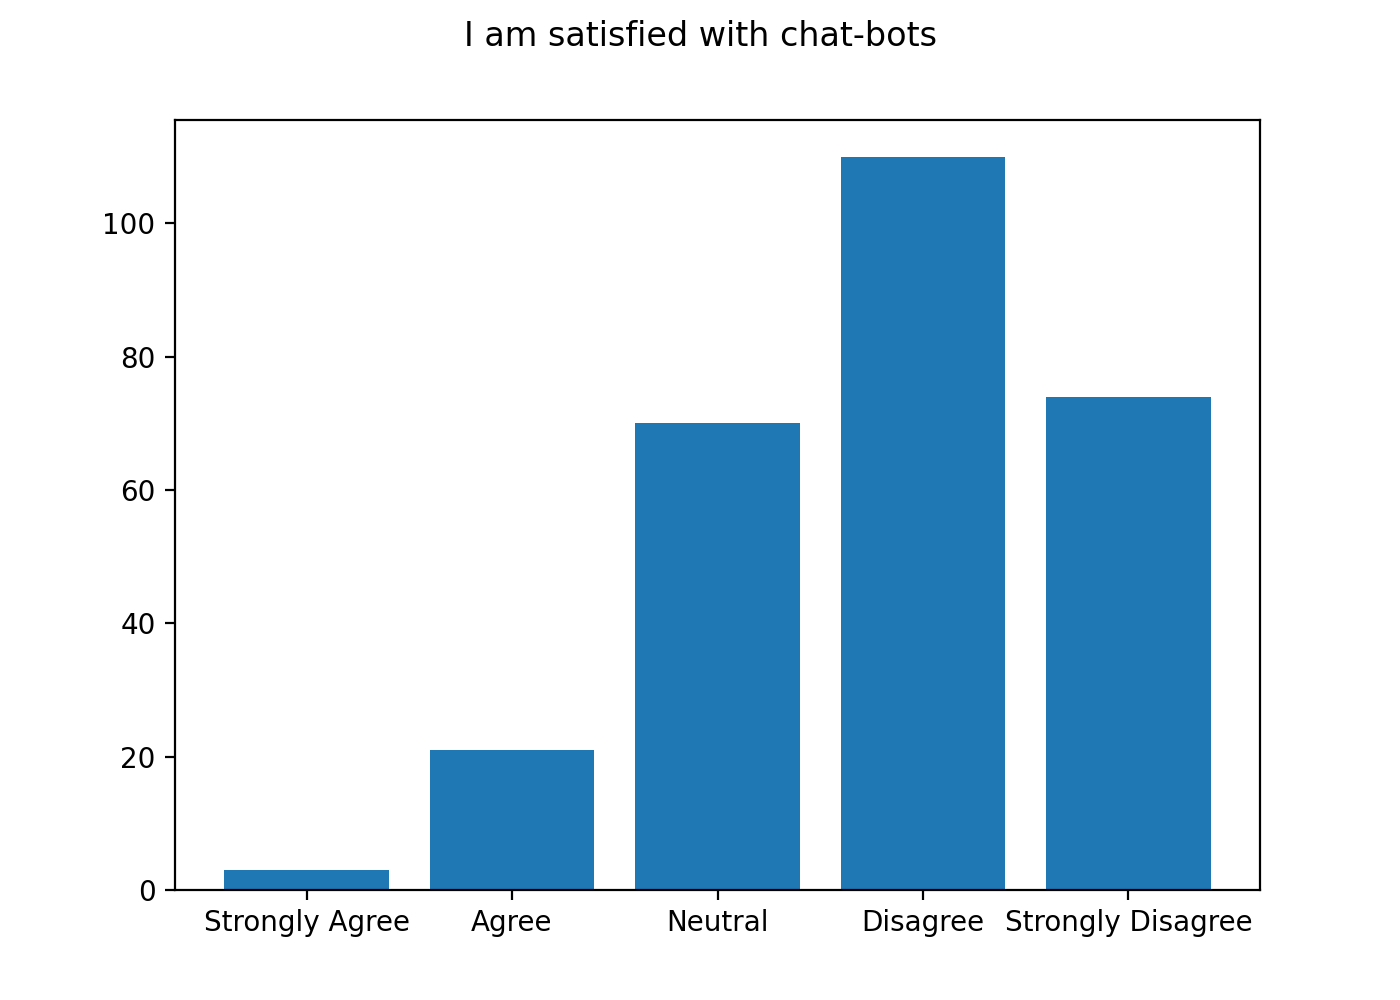
\includegraphics[width=0.6\textwidth,height=\textheight,keepaspectratio]{survey/8_i_am_satisfied_with_chat-bots.png}
}    

Additionally, we can observe higher trust to human employees over automated solutions.

\mtfigure
{Client trust towards interlocutor}
{Own study}
{
    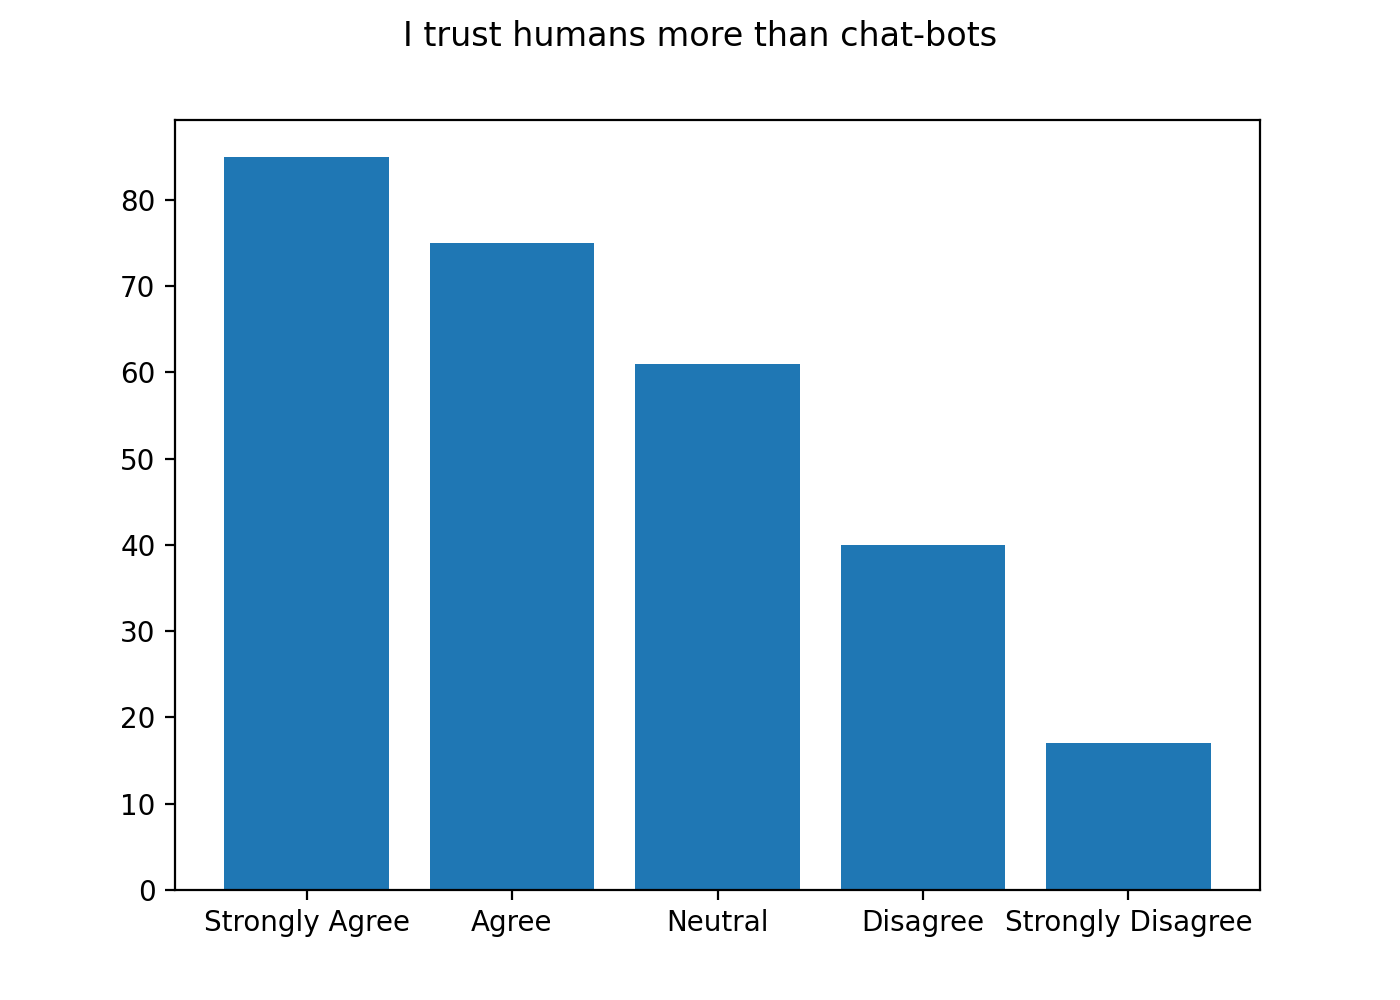
\includegraphics[width=0.6\textwidth,height=\textheight,keepaspectratio]{survey/9_i_trust_humans_more_than_chat-bots.png}
}

As a result, survey showed a lot of interesting points and formed multiple conclusions.
In general, survey showed that people between 18 and 32 years old prefer dialog interfaces over vocal communication.
Moreover, clients will prefer dialog forms over other forms even though those are not as effective as clients expect and may result in slightly negative experience for client.
On the opposite, common argument of long response time may be outdated, as even more demanding generation of clients are neutral.

Although, dialog is preferred, clients tend to trust people more.
In my opinion, this opinion is very subjective, as automated solutions may advise more exactly and don't require prior experience.
Probably, this is connected to high dissatisfaction with existing chatbots' effectiveness.
Moreover, negative impact of chatbots forced clients to learn to determine when they talk to a chatbot and when to an employee.
This results in a strong client association that chatbots are bad and effective.

Consequently, next generation of chatbots have to speak to clients in a natural language, in order to be indistinguishable from employee.
Thus, Artificial Intelligence technologies, including Machine Learning and Natural Language Programming are highly required.

Nevertheless, we can observe general minor satisfaction with existing form of user interaction and negative expectations about automated solutions.
This shows that clients are not ready for chatbots yet.
Moreover, it is possible to conclude that chatbots are not that much for consumers, as they are an important evolution milestone for the banks.

Even if there would be a chatbot solution which passes some limited version of Turing test, when the customer finds
out that all that he was talking to a chatbot, he may feel deceived and lost trust to a bank.

The main hypothesis of this thesis was that Commercial Banking clients are ready for Automated Front Offices in a form of a chatbot.
Conclusively, this hypothesis has to be rejected.
People are not ready and have negative subjective feelings towards chatbots.
Changing those feelings would require significant marketing costs.

However, the most valid injection of a chatbot solution would be in a hybrid approach.
Hybrid approach is a synergy between human employee and an automated chatbot system.
In hybrid approach robot recommends an answer to an operator based on existing knowledge base.
In this case, customer trusts and employee, but receives exact fast answer from an internal chatbot system.

% Conclusion
% !TeX root = ../master_thesis.tex

\unnumberedchapter{Conclusions}

The main trend in commercial banking for the last decade is openness and availability.
Even though, from a regulatory perspective, forcing banks to allow third-party services to operate with a bank in a digital way is a form to divide natural monopolies, openness and availability is highly important on banking market by themselves.
The market of information systems, services and technologies is in all-time high and, obviously, affects such a giant as a banking market.
Banks by its structure are stable and fundamental, which is a logical barrier against extensive development and changes.
Nevertheless, an exponential growth of digital fields is a catalyst for evolution of a banking market.

Nowadays, commercial banks do both front-office and back-office work.
Famous banking stability and guarantees are good for back-office, but can be a massive hurdle in a front-office.
Front-office, as a form of client interaction, has to change as fast as possible in order to achieve its client, client's needs and purposes.
Especially, when entire human ecosystem creates new forms of people communication and interaction.
Extrapolating last two decades we can expect future development of both banking openness and world digitalization.
Accordingly, banks have to adapt to those changes.

Currently, two trends, two forms of bank evolution are formulating — Bank-as-a-Service and Bank-as-a-Platform.
Bank-as-a-Service in a final form makes from a bank a back-office only construct, whose customers are various financial services, which can be risky, can experiment and are not too big to fall.
Although, this form reminds of factoring, it is not.
In spite, those third-party financial services can create their own front-offices, and can operate in fields, which are not available to common bank, in a such way that clients even don't know in which banks their accounts and loans are.
Bank-as-a-Platform, oppositely, is a center, which unites other third-party financial services under its hood and brandname.

Therefore, due to technology development, digitalizaton banks need new forms of interaction.
Moreover, younger generation is known to be more textual, messenger-friendly, and often voice interaction impacts negatively.
Among possibilities, one of the most efficient is a chat-bot.
From customer perspective chat-bot allows solving problems without spending time on waiting for a customer service and without repeating same question towards multiple consultants.
From the banking side, more simple chat-bots decrease costs on customer service and open the possibility to transfer hired employees into less digital fields that require specialization.
Furthermore, the same instrument may significantly increase client engagement and offer growth mechanisms.
On the other hand, in order to achieve client engagement and use mentioned growth mechanisms, bank has to take a massive amount of risk and costs.

Regardless, banking sector should use openness trend and entire digital evolution in order to be in the market.
Moving towards Open Banking helps banking to share work and risks in client interaction.
Consequently, mentioned Machine Learning based chat-bots can be done entirely by third-party providers and supported by them, if there are proper instruments done by bank that allows those to use.
On the other side, third-party providers may not be able to do it entirely, but can offer certain blocks of logic.
In this case, a bank has to build a chat-bot and invest, but with the help of third-party partners.
For a bank mentioned system would be a beautiful piece of a technology, a state-of-art, even though it will require lots of investments and time.

In my opinion, division of labour in banking sector is inevitable.
Unfortunately, it is impossible to know which way would banks develop, towards Banks-as-a-Platform or towards Banks-as-a-Service.

In both options banks have to make actions towards smart textual forms of client communication.
The point is to develop solution iteratively.
Firstly, in all cases banks have to move to even Opener Banking and create even more extensive API.
After that, banks can choose which way do they want to go, either to use already existing solution and integrate with their systems, or to create something entirely new with the latest technologies available.
Integrating existing, more simple rule-based solutions without Artificial Intelligence is an efficient form of interaction due to the fact that entire chat-bot industry is still emerging.
On the other side, creating own Chat-bot with Artifical Intelligence, Machine Learning and Natural Language Processing is an insecure choice, possible for large banks, but definitely extremelly dangerous for small- and medium-sized banks.
Therefore, building chat-bots via third-party development companies as solutions on premise would be the most balanced way of development of this interaction.


% Literature
% !TeX root = ../master_thesis.tex

\begin{spacing}{1.0}
    \printbibliography
    \addcontentsline{toc}{chapter}{BIBLIOGRAPHY}
\end{spacing}


% Appendices
% !TeX root = ../master_thesis.tex

\unnumberedchapter{List of appendices}

\begin{listofshorts}
    \short{AI}{Artificial Intelligence}
    \short{ML}{Machine Learning}
    \short{NLP}{Natural Language Programming}
    \short{NLU}{Natural Language Understanding}
    \short{NLG}{Natural Language Generation}
    \short{GDPR}{General Data Protection Regulation}
    \short{EBA}{European Banking Authority}
    \short{CMA}{Competition and Markets Authority}
    \short{OBIE}{Open Banking Implementation Entity}
    \short{PSD}{Payment Service Directive, first edition}
    \short{PSD2}{Payment Service Directive, second edition}
    \short{ASPSP}{Account Servicing Payment Service Provider}
    \short{TPP}{Third-Party Provider}
    \short{AISP}{Account Information Service Provider}
    \short{PISP}{Payment Initiation Service Provider}
    \short{PIISP}{Payment Instrument Issuer Service Provider}
    \short{SCA}{Strong Customer Authentication}
    \short{PSU}{Payment Service User}
    \short{DBMS}{Database Management System}
    \short{MBMS}{Model Base Management System}
    \short{CV}{Curriculum Vitae}
    \short{MiFID II}{Markets in Financial Instruments Directive, second edition}
    \short{R\&D}{Research and Development}
    \short{KYC}{Know Your Customer}
    \short{AML}{Anti-Money Laundering}
    \short{API}{Application Programming Interface}
    \short{BaaS}{Banking-as-a-Service}
    \short{BaaP}{Banking-as-a-Platform}
    \short{CRM}{Customer Relationship Management}
\end{listofshorts}

\listoftables

\listoffigures

\listofannexes

\end{document}
